% Options for packages loaded elsewhere
\PassOptionsToPackage{unicode}{hyperref}
\PassOptionsToPackage{hyphens}{url}
%
\documentclass[
]{article}
\usepackage{amsmath,amssymb}
\usepackage{iftex}
\ifPDFTeX
  \usepackage[T1]{fontenc}
  \usepackage[utf8]{inputenc}
  \usepackage{textcomp} % provide euro and other symbols
\else % if luatex or xetex
  \usepackage{unicode-math} % this also loads fontspec
  \defaultfontfeatures{Scale=MatchLowercase}
  \defaultfontfeatures[\rmfamily]{Ligatures=TeX,Scale=1}
\fi
\usepackage{lmodern}
\ifPDFTeX\else
  % xetex/luatex font selection
\fi
% Use upquote if available, for straight quotes in verbatim environments
\IfFileExists{upquote.sty}{\usepackage{upquote}}{}
\IfFileExists{microtype.sty}{% use microtype if available
  \usepackage[]{microtype}
  \UseMicrotypeSet[protrusion]{basicmath} % disable protrusion for tt fonts
}{}
\makeatletter
\@ifundefined{KOMAClassName}{% if non-KOMA class
  \IfFileExists{parskip.sty}{%
    \usepackage{parskip}
  }{% else
    \setlength{\parindent}{0pt}
    \setlength{\parskip}{6pt plus 2pt minus 1pt}}
}{% if KOMA class
  \KOMAoptions{parskip=half}}
\makeatother
\usepackage{xcolor}
\usepackage[margin=1in]{geometry}
\usepackage{color}
\usepackage{fancyvrb}
\newcommand{\VerbBar}{|}
\newcommand{\VERB}{\Verb[commandchars=\\\{\}]}
\DefineVerbatimEnvironment{Highlighting}{Verbatim}{commandchars=\\\{\}}
% Add ',fontsize=\small' for more characters per line
\usepackage{framed}
\definecolor{shadecolor}{RGB}{248,248,248}
\newenvironment{Shaded}{\begin{snugshade}}{\end{snugshade}}
\newcommand{\AlertTok}[1]{\textcolor[rgb]{0.94,0.16,0.16}{#1}}
\newcommand{\AnnotationTok}[1]{\textcolor[rgb]{0.56,0.35,0.01}{\textbf{\textit{#1}}}}
\newcommand{\AttributeTok}[1]{\textcolor[rgb]{0.13,0.29,0.53}{#1}}
\newcommand{\BaseNTok}[1]{\textcolor[rgb]{0.00,0.00,0.81}{#1}}
\newcommand{\BuiltInTok}[1]{#1}
\newcommand{\CharTok}[1]{\textcolor[rgb]{0.31,0.60,0.02}{#1}}
\newcommand{\CommentTok}[1]{\textcolor[rgb]{0.56,0.35,0.01}{\textit{#1}}}
\newcommand{\CommentVarTok}[1]{\textcolor[rgb]{0.56,0.35,0.01}{\textbf{\textit{#1}}}}
\newcommand{\ConstantTok}[1]{\textcolor[rgb]{0.56,0.35,0.01}{#1}}
\newcommand{\ControlFlowTok}[1]{\textcolor[rgb]{0.13,0.29,0.53}{\textbf{#1}}}
\newcommand{\DataTypeTok}[1]{\textcolor[rgb]{0.13,0.29,0.53}{#1}}
\newcommand{\DecValTok}[1]{\textcolor[rgb]{0.00,0.00,0.81}{#1}}
\newcommand{\DocumentationTok}[1]{\textcolor[rgb]{0.56,0.35,0.01}{\textbf{\textit{#1}}}}
\newcommand{\ErrorTok}[1]{\textcolor[rgb]{0.64,0.00,0.00}{\textbf{#1}}}
\newcommand{\ExtensionTok}[1]{#1}
\newcommand{\FloatTok}[1]{\textcolor[rgb]{0.00,0.00,0.81}{#1}}
\newcommand{\FunctionTok}[1]{\textcolor[rgb]{0.13,0.29,0.53}{\textbf{#1}}}
\newcommand{\ImportTok}[1]{#1}
\newcommand{\InformationTok}[1]{\textcolor[rgb]{0.56,0.35,0.01}{\textbf{\textit{#1}}}}
\newcommand{\KeywordTok}[1]{\textcolor[rgb]{0.13,0.29,0.53}{\textbf{#1}}}
\newcommand{\NormalTok}[1]{#1}
\newcommand{\OperatorTok}[1]{\textcolor[rgb]{0.81,0.36,0.00}{\textbf{#1}}}
\newcommand{\OtherTok}[1]{\textcolor[rgb]{0.56,0.35,0.01}{#1}}
\newcommand{\PreprocessorTok}[1]{\textcolor[rgb]{0.56,0.35,0.01}{\textit{#1}}}
\newcommand{\RegionMarkerTok}[1]{#1}
\newcommand{\SpecialCharTok}[1]{\textcolor[rgb]{0.81,0.36,0.00}{\textbf{#1}}}
\newcommand{\SpecialStringTok}[1]{\textcolor[rgb]{0.31,0.60,0.02}{#1}}
\newcommand{\StringTok}[1]{\textcolor[rgb]{0.31,0.60,0.02}{#1}}
\newcommand{\VariableTok}[1]{\textcolor[rgb]{0.00,0.00,0.00}{#1}}
\newcommand{\VerbatimStringTok}[1]{\textcolor[rgb]{0.31,0.60,0.02}{#1}}
\newcommand{\WarningTok}[1]{\textcolor[rgb]{0.56,0.35,0.01}{\textbf{\textit{#1}}}}
\usepackage{graphicx}
\makeatletter
\def\maxwidth{\ifdim\Gin@nat@width>\linewidth\linewidth\else\Gin@nat@width\fi}
\def\maxheight{\ifdim\Gin@nat@height>\textheight\textheight\else\Gin@nat@height\fi}
\makeatother
% Scale images if necessary, so that they will not overflow the page
% margins by default, and it is still possible to overwrite the defaults
% using explicit options in \includegraphics[width, height, ...]{}
\setkeys{Gin}{width=\maxwidth,height=\maxheight,keepaspectratio}
% Set default figure placement to htbp
\makeatletter
\def\fps@figure{htbp}
\makeatother
\setlength{\emergencystretch}{3em} % prevent overfull lines
\providecommand{\tightlist}{%
  \setlength{\itemsep}{0pt}\setlength{\parskip}{0pt}}
\setcounter{secnumdepth}{-\maxdimen} % remove section numbering
\usepackage{amsmath}
\ifLuaTeX
  \usepackage{selnolig}  % disable illegal ligatures
\fi
\usepackage{bookmark}
\IfFileExists{xurl.sty}{\usepackage{xurl}}{} % add URL line breaks if available
\urlstyle{same}
\hypersetup{
  pdftitle={Adaptive Sampling simulations},
  pdfauthor={Corey Williams},
  hidelinks,
  pdfcreator={LaTeX via pandoc}}

\title{Adaptive Sampling simulations}
\author{Corey Williams}
\date{2024-05-16}

\begin{document}
\maketitle

{
\setcounter{tocdepth}{2}
\tableofcontents
}
\section{Motivation for adaptive
sampling}\label{motivation-for-adaptive-sampling}

In many scenarios we would like to be able to adaptively increase
sampling effort when certain observed values are of interest. This would
be especially beneficial in the case where we are try to observe rare
events that are likely to be clustered together. For example a rare
plant species that has very particular growing conditions. This would be
the case where it may be very rare to see the plant but if we see one we
see 100 and it is desired to be able to sample all of the plants in the
cluster.

\section{Simulations}\label{simulations}

First I'll write a few functions that I think will be helpful in making
this adaptive sampling demonstration. I want to recreate the example in
Adaptive cluster Sampling (1990) where there are points distributed in
clusters in an area. The area is split into a grid, then grid cells are
chosen as the primary sampling unit.

Goals:

\begin{itemize}
\tightlist
\item
  choose a number of clusters

  \begin{itemize}
  \tightlist
  \item
    easy enough, this can just be rpois(1,n), this will choose a number
    of clusters randomly based on some mean. We could use any discrete
    distribution to decide this
  \end{itemize}
\item
  generate points in those clusters

  \begin{itemize}
  \tightlist
  \item
    decide how many points are in each cluster, this it is probably
    actually most appropriate to use a poisson distribution since it
    will be a count.
  \end{itemize}
\item
  at this step I also need to choose the locations of the centers,
  runif(ncenters,0,20)
\item
  I can then generate points normally distributed around these centers
  using rnorm(ncenters*2,mu,sd)
\item
  choose a sample of initial grid cells

  \begin{itemize}
  \tightlist
  \item
    sample(1:ncells,n)
  \end{itemize}
\item
  expand if the cell next to it is occupied

  \begin{itemize}
  \tightlist
  \item
    need a list of currently occupied cells and a way to determine
    adjacent cells. maybe just a vector called occupied
  \item
    function takes vector of neighbours, checks against vector of
    occupied, returns neighbors in occupied
  \end{itemize}
\end{itemize}

\section{Creating functions for
sampling}\label{creating-functions-for-sampling}

\begin{Shaded}
\begin{Highlighting}[]
\FunctionTok{require}\NormalTok{(tidyverse) }\CommentTok{\# for plotting, dply data manipulation, and maps from purrr}
\end{Highlighting}
\end{Shaded}

\begin{verbatim}
## Loading required package: tidyverse
\end{verbatim}

\begin{verbatim}
## -- Attaching core tidyverse packages ------------------------ tidyverse 2.0.0 --
## v dplyr     1.1.4     v readr     2.1.5
## v forcats   1.0.0     v stringr   1.5.1
## v ggplot2   3.5.1     v tibble    3.2.1
## v lubridate 1.9.3     v tidyr     1.3.1
## v purrr     1.0.2     
## -- Conflicts ------------------------------------------ tidyverse_conflicts() --
## x dplyr::filter() masks stats::filter()
## x dplyr::lag()    masks stats::lag()
## i Use the conflicted package (<http://conflicted.r-lib.org/>) to force all conflicts to become errors
\end{verbatim}

\begin{Shaded}
\begin{Highlighting}[]
\CommentTok{\# install.packages("ggridges")}
\FunctionTok{require}\NormalTok{(ggridges) }\CommentTok{\# creating nice plots of simulation results}
\end{Highlighting}
\end{Shaded}

\begin{verbatim}
## Loading required package: ggridges
\end{verbatim}

\begin{Shaded}
\begin{Highlighting}[]
\CommentTok{\# install.packages("colorspace")}
\CommentTok{\# require(colorspace)}
\end{Highlighting}
\end{Shaded}

\subsubsection{make clusters}\label{make-clusters}

\begin{Shaded}
\begin{Highlighting}[]
\NormalTok{make\_clusters}\OtherTok{\textless{}{-}}\ControlFlowTok{function}\NormalTok{(}\AttributeTok{grid\_size=}\DecValTok{20}\NormalTok{, }\AttributeTok{nclusters=}\DecValTok{3}\NormalTok{, }\AttributeTok{avg\_size=}\DecValTok{20}\NormalTok{, }\AttributeTok{force\_inclusion=}\ConstantTok{FALSE}\NormalTok{)\{}
  \CommentTok{\# create a list of clusters.}
\NormalTok{  centers}\OtherTok{\textless{}{-}}\FunctionTok{split}\NormalTok{(}\FunctionTok{runif}\NormalTok{(nclusters}\SpecialCharTok{*}\DecValTok{2}\NormalTok{,}\DecValTok{0}\NormalTok{,grid\_size),}\FunctionTok{seq}\NormalTok{(nclusters))}
  \CommentTok{\# get the three cluster sizes}
\NormalTok{  sizes}\OtherTok{\textless{}{-}}\FunctionTok{rpois}\NormalTok{(}\DecValTok{3}\NormalTok{,avg\_size)}
  \CommentTok{\# get list of matrices of the centers}
\NormalTok{  center\_dfs}\OtherTok{\textless{}{-}}\FunctionTok{map2}\NormalTok{(sizes,centers,}
                   \SpecialCharTok{\textasciitilde{}} \FunctionTok{kronecker}\NormalTok{(}\FunctionTok{matrix}\NormalTok{(}\FunctionTok{rep}\NormalTok{(}\DecValTok{1}\NormalTok{,.x),}\AttributeTok{ncol=}\DecValTok{1}\NormalTok{), }\FunctionTok{matrix}\NormalTok{(.y,}\AttributeTok{ncol=}\DecValTok{2}\NormalTok{)))}
                              \CommentTok{\# I actually used the kronecker product holy crap!}
  
  \ControlFlowTok{if}\NormalTok{(force\_inclusion}\SpecialCharTok{==}\NormalTok{T)\{}
    \CommentTok{\# get coordinates of locations}
\NormalTok{    locations}\OtherTok{\textless{}{-}}\NormalTok{sizes }\SpecialCharTok{\%\textgreater{}\%} \CommentTok{\# use sizes}
      \FunctionTok{map}\NormalTok{( }\SpecialCharTok{\textasciitilde{}}\FunctionTok{data.frame}\NormalTok{(}\FunctionTok{matrix}\NormalTok{(}\FunctionTok{rnorm}\NormalTok{(.x}\SpecialCharTok{*}\DecValTok{2}\NormalTok{),}\AttributeTok{ncol=}\DecValTok{2}\NormalTok{))) }\SpecialCharTok{\%\textgreater{}\%} \CommentTok{\# make list of df of changes from centers}
      \FunctionTok{map2}\NormalTok{(}\AttributeTok{.y=}\NormalTok{center\_dfs, }\SpecialCharTok{\textasciitilde{}}\NormalTok{.x}\SpecialCharTok{+}\NormalTok{.y) }\SpecialCharTok{\%\textgreater{}\%} \CommentTok{\# add the changes on to the center}
      \FunctionTok{map2}\NormalTok{(}\AttributeTok{.y=}\FunctionTok{seq}\NormalTok{(nclusters), }\SpecialCharTok{\textasciitilde{}} \FunctionTok{mutate}\NormalTok{(.x, }\AttributeTok{Group=}\FunctionTok{paste}\NormalTok{(}\StringTok{"Cluster"}\NormalTok{,.y)))}\SpecialCharTok{\%\textgreater{}\%}
      \FunctionTok{bind\_rows}\NormalTok{()}
    \FunctionTok{colnames}\NormalTok{(locations)}\OtherTok{\textless{}{-}}\FunctionTok{c}\NormalTok{(}\StringTok{"X"}\NormalTok{,}\StringTok{"Y"}\NormalTok{,}\StringTok{"Group"}\NormalTok{)}
    \CommentTok{\# force points to snap inside if they were generated outside. This means some}
    \CommentTok{\# tiles will be more densely clustered at edges when a center is near an edge}
    \CommentTok{\# should help maintain the average number of points though}
\NormalTok{    locations}\OtherTok{\textless{}{-}}\NormalTok{locations}\SpecialCharTok{\%\textgreater{}\%}
      \FunctionTok{mutate}\NormalTok{(}\AttributeTok{X=}\FunctionTok{ifelse}\NormalTok{(X}\SpecialCharTok{\textgreater{}}\NormalTok{grid\_size,grid\_size,X))}\SpecialCharTok{\%\textgreater{}\%}
      \FunctionTok{mutate}\NormalTok{(}\AttributeTok{X=}\FunctionTok{ifelse}\NormalTok{(X}\SpecialCharTok{\textless{}}\DecValTok{0}\NormalTok{, }\DecValTok{0}\NormalTok{, X))}\SpecialCharTok{\%\textgreater{}\%}
      \FunctionTok{mutate}\NormalTok{(}\AttributeTok{Y=}\FunctionTok{ifelse}\NormalTok{(Y}\SpecialCharTok{\textgreater{}}\NormalTok{grid\_size,grid\_size,Y))}\SpecialCharTok{\%\textgreater{}\%}
      \FunctionTok{mutate}\NormalTok{(}\AttributeTok{Y=}\FunctionTok{ifelse}\NormalTok{(Y}\SpecialCharTok{\textless{}}\DecValTok{0}\NormalTok{, }\DecValTok{0}\NormalTok{, Y))}
      
\NormalTok{  \}}\ControlFlowTok{else}\NormalTok{\{}
    \CommentTok{\# get coordinates of locations}
\NormalTok{    locations}\OtherTok{\textless{}{-}}\NormalTok{sizes }\SpecialCharTok{\%\textgreater{}\%} \CommentTok{\# use sizes}
      \FunctionTok{map}\NormalTok{(}\SpecialCharTok{\textasciitilde{}}\FunctionTok{data.frame}\NormalTok{(}\FunctionTok{matrix}\NormalTok{(}\FunctionTok{rnorm}\NormalTok{(.x}\SpecialCharTok{*}\DecValTok{2}\NormalTok{),}\AttributeTok{ncol=}\DecValTok{2}\NormalTok{))) }\SpecialCharTok{\%\textgreater{}\%} \CommentTok{\# make list of df of changes from centers}
      \FunctionTok{map2}\NormalTok{(}\AttributeTok{.y=}\NormalTok{center\_dfs,}\SpecialCharTok{\textasciitilde{}}\NormalTok{.x}\SpecialCharTok{+}\NormalTok{.y) }\SpecialCharTok{\%\textgreater{}\%} \CommentTok{\# add the changes on to the center}
      \FunctionTok{map2}\NormalTok{(}\AttributeTok{.y=}\FunctionTok{seq}\NormalTok{(nclusters), }\SpecialCharTok{\textasciitilde{}} \FunctionTok{mutate}\NormalTok{(.x, }\AttributeTok{Group=}\FunctionTok{paste}\NormalTok{(}\StringTok{"Cluster"}\NormalTok{,.y)))}\SpecialCharTok{\%\textgreater{}\%}
      \FunctionTok{bind\_rows}\NormalTok{()}
    \FunctionTok{colnames}\NormalTok{(locations)}\OtherTok{\textless{}{-}}\FunctionTok{c}\NormalTok{(}\StringTok{"X"}\NormalTok{,}\StringTok{"Y"}\NormalTok{,}\StringTok{"Group"}\NormalTok{)}
\NormalTok{  \}}
\NormalTok{  locations}
\NormalTok{\}}
\FunctionTok{head}\NormalTok{(}\FunctionTok{make\_clusters}\NormalTok{(}\AttributeTok{force\_inclusion =} \ConstantTok{TRUE}\NormalTok{))}
\end{Highlighting}
\end{Shaded}

\begin{verbatim}
##          X        Y     Group
## 1 19.50915 14.66253 Cluster 1
## 2 19.70652 13.63672 Cluster 1
## 3 20.00000 14.30465 Cluster 1
## 4 19.88728 13.13993 Cluster 1
## 5 20.00000 15.08183 Cluster 1
## 6 20.00000 14.05885 Cluster 1
\end{verbatim}

\subsubsection{plotting}\label{plotting}

\begin{Shaded}
\begin{Highlighting}[]
\NormalTok{plot\_clusters}\OtherTok{\textless{}{-}}\ControlFlowTok{function}\NormalTok{(cluster\_df, }\AttributeTok{grid\_size=}\DecValTok{20}\NormalTok{,}\AttributeTok{samp=}\ConstantTok{NULL}\NormalTok{)\{}
  \CommentTok{\# cluster\_df is the set of points on the grid}
  \CommentTok{\# samp is the set of tiles that were sampled}
  \CommentTok{\# create a plot of the clusters}
\NormalTok{  p}\OtherTok{\textless{}{-}}\FunctionTok{ggplot}\NormalTok{(cluster\_df, }\FunctionTok{aes}\NormalTok{(}\AttributeTok{x=}\NormalTok{X, }\AttributeTok{y=}\NormalTok{Y, }\AttributeTok{color=}\NormalTok{Group))}\SpecialCharTok{+}
    \FunctionTok{geom\_point}\NormalTok{()}\SpecialCharTok{+}
    \FunctionTok{scale\_x\_continuous}\NormalTok{(}\AttributeTok{breaks=}\FunctionTok{seq}\NormalTok{(grid\_size))}\SpecialCharTok{+}
    \FunctionTok{scale\_y\_continuous}\NormalTok{(}\AttributeTok{breaks=}\FunctionTok{seq}\NormalTok{(grid\_size))}\SpecialCharTok{+}
    \FunctionTok{coord\_cartesian}\NormalTok{(}\AttributeTok{xlim=}\FunctionTok{c}\NormalTok{(}\DecValTok{0}\NormalTok{,grid\_size), }\AttributeTok{ylim=}\FunctionTok{c}\NormalTok{(}\DecValTok{0}\NormalTok{,grid\_size))}
  \ControlFlowTok{if}\NormalTok{(}\SpecialCharTok{!}\FunctionTok{is.null}\NormalTok{(samp))\{}
    \CommentTok{\# this will highlight tiles that are sampled}
    \CommentTok{\# samp is the dataframe containing the coordinates for tiles}
\NormalTok{    p}\OtherTok{\textless{}{-}}\NormalTok{p}\SpecialCharTok{+}\FunctionTok{geom\_rect}\NormalTok{(}\AttributeTok{data=}\NormalTok{samp, }
                   \FunctionTok{aes}\NormalTok{( }\AttributeTok{xmin=}\NormalTok{X}\DecValTok{{-}1}\NormalTok{, }\AttributeTok{xmax=}\NormalTok{X, }\AttributeTok{ymin=}\NormalTok{Y}\DecValTok{{-}1}\NormalTok{, }\AttributeTok{ymax=}\NormalTok{Y),}
                   \AttributeTok{color=}\StringTok{"black"}\NormalTok{,}
                   \AttributeTok{fill=}\ConstantTok{NA}\NormalTok{)}
\NormalTok{  \}}
  \FunctionTok{plot}\NormalTok{(p)}
\NormalTok{\}}
\end{Highlighting}
\end{Shaded}

\subsubsection{Check whether a tile is
occupied}\label{check-whether-a-tile-is-occupied}

\begin{Shaded}
\begin{Highlighting}[]
\NormalTok{is\_occupied}\OtherTok{\textless{}{-}}\ControlFlowTok{function}\NormalTok{(}\AttributeTok{tile=}\FunctionTok{c}\NormalTok{(}\DecValTok{1}\NormalTok{,}\DecValTok{1}\NormalTok{,}\DecValTok{1}\NormalTok{),df)\{}
  \CommentTok{\# check if a tile is occupied tile location is given as c(row,column)}
  \CommentTok{\# give a dataframe with coordinates of point}
  \CommentTok{\# check if there are any points in xrange \& yrange at the same time}
  \CommentTok{\#sum((df[,1]\textless{}tile[2] \& df[,1]\textgreater{}tile[2]{-}1) * (df[,1]\textless{}tile[2] \& df[,1]\textgreater{}tile[2]{-}1))\textgreater{}0}
  
  \FunctionTok{sum}\NormalTok{((df[,}\DecValTok{1}\NormalTok{]}\SpecialCharTok{\textless{}}\NormalTok{tile[}\DecValTok{1}\NormalTok{]}\SpecialCharTok{\&}\NormalTok{df[,}\DecValTok{1}\NormalTok{]}\SpecialCharTok{\textgreater{}}\NormalTok{tile[}\DecValTok{1}\NormalTok{]}\SpecialCharTok{{-}}\DecValTok{1}\NormalTok{) }\SpecialCharTok{\&}\NormalTok{ (df[,}\DecValTok{2}\NormalTok{]}\SpecialCharTok{\textless{}}\NormalTok{tile[}\DecValTok{2}\NormalTok{] }\SpecialCharTok{\&}\NormalTok{ df[,}\DecValTok{2}\NormalTok{]}\SpecialCharTok{\textgreater{}}\NormalTok{tile[}\DecValTok{2}\NormalTok{]}\SpecialCharTok{{-}}\DecValTok{1}\NormalTok{))}\SpecialCharTok{\textgreater{}}\DecValTok{0}
\NormalTok{\}}
\end{Highlighting}
\end{Shaded}

\paragraph{find the average in a single
tile}\label{find-the-average-in-a-single-tile}

this will get used in the hansen hurwitz estimator as well. Just
including it here so we can have y\_k in the simulated data.

\begin{Shaded}
\begin{Highlighting}[]
\NormalTok{tile\_sum}\OtherTok{\textless{}{-}}\ControlFlowTok{function}\NormalTok{(}\AttributeTok{tile=}\FunctionTok{c}\NormalTok{(}\AttributeTok{X=}\DecValTok{1}\NormalTok{,}\AttributeTok{Y=}\DecValTok{1}\NormalTok{,}\AttributeTok{K=}\DecValTok{1}\NormalTok{), df)\{}
  \CommentTok{\# This function returns the y\_k for tile k}
  \CommentTok{\# tile is the tile to find the response of }
  \CommentTok{\# df is the dataframe of points on the grid}
  \FunctionTok{sum}\NormalTok{((df[,}\DecValTok{1}\NormalTok{]}\SpecialCharTok{\textless{}}\NormalTok{tile[}\DecValTok{1}\NormalTok{]}\SpecialCharTok{\&}\NormalTok{df[,}\DecValTok{1}\NormalTok{]}\SpecialCharTok{\textgreater{}}\NormalTok{tile[}\DecValTok{1}\NormalTok{]}\SpecialCharTok{{-}}\DecValTok{1}\NormalTok{) }\SpecialCharTok{\&}\NormalTok{ (df[,}\DecValTok{2}\NormalTok{]}\SpecialCharTok{\textless{}}\NormalTok{tile[}\DecValTok{2}\NormalTok{] }\SpecialCharTok{\&}\NormalTok{ df[,}\DecValTok{2}\NormalTok{]}\SpecialCharTok{\textgreater{}}\NormalTok{tile[}\DecValTok{2}\NormalTok{]}\SpecialCharTok{{-}}\DecValTok{1}\NormalTok{))}
\NormalTok{\}}
\end{Highlighting}
\end{Shaded}

\subsubsection{get the neighbours of a
tile}\label{get-the-neighbours-of-a-tile}

\begin{Shaded}
\begin{Highlighting}[]
\NormalTok{get\_neighbours}\OtherTok{\textless{}{-}} \ControlFlowTok{function}\NormalTok{(}\AttributeTok{tile=}\FunctionTok{c}\NormalTok{(}\AttributeTok{X=}\DecValTok{1}\NormalTok{,}\AttributeTok{Y=}\DecValTok{1}\NormalTok{,}\AttributeTok{k=}\DecValTok{1}\NormalTok{), }\AttributeTok{hard\_border=}\ConstantTok{TRUE}\NormalTok{,}\AttributeTok{grid\_size=}\DecValTok{20}\NormalTok{)\{}
  \CommentTok{\# gets a list of neighbouring tiles}
\NormalTok{  neighbours}\OtherTok{\textless{}{-}}\FunctionTok{list}\NormalTok{(}\FunctionTok{c}\NormalTok{(tile[}\DecValTok{1}\NormalTok{]}\SpecialCharTok{{-}}\DecValTok{1}\NormalTok{, tile[}\DecValTok{2}\NormalTok{],   tile[}\DecValTok{3}\NormalTok{]),}
                   \FunctionTok{c}\NormalTok{(tile[}\DecValTok{1}\NormalTok{],   tile[}\DecValTok{2}\NormalTok{]}\SpecialCharTok{{-}}\DecValTok{1}\NormalTok{, tile[}\DecValTok{3}\NormalTok{]),}
                   \FunctionTok{c}\NormalTok{(tile[}\DecValTok{1}\NormalTok{]}\SpecialCharTok{+}\DecValTok{1}\NormalTok{, tile[}\DecValTok{2}\NormalTok{],   tile[}\DecValTok{3}\NormalTok{]),}
                   \FunctionTok{c}\NormalTok{(tile[}\DecValTok{1}\NormalTok{],   tile[}\DecValTok{2}\NormalTok{]}\SpecialCharTok{+}\DecValTok{1}\NormalTok{, tile[}\DecValTok{3}\NormalTok{]))}
  \ControlFlowTok{if}\NormalTok{(hard\_border)\{}
    \CommentTok{\# do we want to include neighbours outside of the grid?}
    \CommentTok{\# returns the neighbours that are only within the border}
\NormalTok{    neighbours}\OtherTok{\textless{}{-}}\NormalTok{neighbours[}\FunctionTok{map\_lgl}\NormalTok{(neighbours, }\SpecialCharTok{\textasciitilde{}}\FunctionTok{prod}\NormalTok{(}\FunctionTok{c}\NormalTok{(.x}\SpecialCharTok{\textgreater{}}\DecValTok{0}\NormalTok{,.x}\SpecialCharTok{\textless{}=}\NormalTok{grid\_size)))]}
\NormalTok{  \}}
  \CommentTok{\# returns list of neighbours for a given tile }
\NormalTok{  neighbours}
\NormalTok{\}}
\end{Highlighting}
\end{Shaded}

\subsubsection{choose tiles for sample}\label{choose-tiles-for-sample}

\begin{Shaded}
\begin{Highlighting}[]
\NormalTok{get\_tiles}\OtherTok{\textless{}{-}}\ControlFlowTok{function}\NormalTok{(}\AttributeTok{grid\_size=}\DecValTok{20}\NormalTok{,}\AttributeTok{n1=}\DecValTok{10}\NormalTok{,...)\{}
  \CommentTok{\# this function returns a sample of n1 tiles using a square grid\_size grid}
  \CommentTok{\# get a tile}
\NormalTok{  tiles}\OtherTok{\textless{}{-}}\FunctionTok{sample}\NormalTok{(}\DecValTok{1}\SpecialCharTok{:}\NormalTok{grid\_size}\SpecialCharTok{\^{}}\DecValTok{2}\NormalTok{,n1,...)}
  \CommentTok{\# convert tile numbers into X and Y}
\NormalTok{  samp}\OtherTok{\textless{}{-}}\FunctionTok{data.frame}\NormalTok{(}\AttributeTok{X=}\NormalTok{tiles}\SpecialCharTok{\%\%}\NormalTok{grid\_size, }\AttributeTok{Y=}\NormalTok{(tiles}\DecValTok{{-}1}\NormalTok{)}\SpecialCharTok{\%/\%}\NormalTok{grid\_size}\SpecialCharTok{+}\DecValTok{1}\NormalTok{)}
\NormalTok{  samp}\SpecialCharTok{$}\NormalTok{X[samp}\SpecialCharTok{$}\NormalTok{X}\SpecialCharTok{==}\DecValTok{0}\NormalTok{]}\OtherTok{\textless{}{-}}\NormalTok{grid\_size}
\NormalTok{  samp}\SpecialCharTok{$}\NormalTok{k}\OtherTok{\textless{}{-}}\DecValTok{1}\SpecialCharTok{:}\NormalTok{n1}
\NormalTok{  samp}
\NormalTok{\}}
\end{Highlighting}
\end{Shaded}

\subsection{Performing adaptive cluster
sampling}\label{performing-adaptive-cluster-sampling}

\subsubsection{One sample from a population of
points}\label{one-sample-from-a-population-of-points}

\begin{Shaded}
\begin{Highlighting}[]
\NormalTok{simulate\_one}\OtherTok{\textless{}{-}}\ControlFlowTok{function}\NormalTok{(}\AttributeTok{nclusters=}\DecValTok{3}\NormalTok{, }\AttributeTok{grid\_size=}\DecValTok{20}\NormalTok{,}\AttributeTok{n1=}\DecValTok{10}\NormalTok{,}\AttributeTok{force\_inclusion=}\ConstantTok{FALSE}\NormalTok{, }\AttributeTok{hard\_border=}\ConstantTok{TRUE}\NormalTok{,... )\{}
  \CommentTok{\# generate clusters}
\NormalTok{  points}\OtherTok{\textless{}{-}}\FunctionTok{make\_clusters}\NormalTok{(}\AttributeTok{force\_inclusion =}\NormalTok{ force\_inclusion)}
  \CommentTok{\# choose the starting grid cells}
\NormalTok{  sample\_tiles}\OtherTok{\textless{}{-}}\FunctionTok{get\_tiles}\NormalTok{(}\AttributeTok{n1=}\DecValTok{10}\NormalTok{,...)}
  \CommentTok{\# save a copy to check against for updates}
\NormalTok{  temp}\OtherTok{\textless{}{-}}\NormalTok{sample\_tiles}
  \CommentTok{\# check whether or not they are occupied based on the clusters}
\NormalTok{  occupied}\OtherTok{\textless{}{-}}\FunctionTok{apply}\NormalTok{(sample\_tiles,}\DecValTok{1}\NormalTok{,}\ControlFlowTok{function}\NormalTok{(x) }\FunctionTok{is\_occupied}\NormalTok{(x, points))}
  \CommentTok{\# find the neighbours of the occupied points}
\NormalTok{  neighbours}\OtherTok{\textless{}{-}}\FunctionTok{apply}\NormalTok{(sample\_tiles[occupied,], }\DecValTok{1}\NormalTok{, }\ControlFlowTok{function}\NormalTok{(x) }\FunctionTok{get\_neighbours}\NormalTok{(x,}\AttributeTok{hard\_border =} \ConstantTok{TRUE}\NormalTok{))}\SpecialCharTok{\%\textgreater{}\%} \CommentTok{\# get neighbours}
    \FunctionTok{bind\_rows}\NormalTok{() }\SpecialCharTok{\%\textgreater{}\%} \CommentTok{\# turn list of neighbours into tibble}
    \FunctionTok{as.data.frame}\NormalTok{() }\CommentTok{\# into dataframe}
  \CommentTok{\# update sample tiles to include neighbours}
\NormalTok{  sample\_tiles}\OtherTok{\textless{}{-}}\FunctionTok{rbind}\NormalTok{(sample\_tiles,neighbours) }\SpecialCharTok{\%\textgreater{}\%}
    \FunctionTok{unique}\NormalTok{()}
  
  \CommentTok{\# keep looping until sample\_tiles does not grow}
  \ControlFlowTok{while}\NormalTok{(}\FunctionTok{dim}\NormalTok{(temp)[}\DecValTok{1}\NormalTok{]}\SpecialCharTok{!=}\FunctionTok{dim}\NormalTok{(sample\_tiles)[}\DecValTok{1}\NormalTok{])\{ }
    \CommentTok{\# save a copy to check against for updates}
\NormalTok{    temp}\OtherTok{\textless{}{-}}\NormalTok{sample\_tiles}
    \CommentTok{\# check whether or not they are occupied based on the clusters}
\NormalTok{    occupied}\OtherTok{\textless{}{-}}\FunctionTok{apply}\NormalTok{(sample\_tiles,}\DecValTok{1}\NormalTok{,}\ControlFlowTok{function}\NormalTok{(x) }\FunctionTok{is\_occupied}\NormalTok{(x,points))}
    \CommentTok{\# find the neighbours of the occupied points}
\NormalTok{    neighbours}\OtherTok{\textless{}{-}}\FunctionTok{apply}\NormalTok{(sample\_tiles[occupied,], }\DecValTok{1}\NormalTok{, }\ControlFlowTok{function}\NormalTok{(x) }\FunctionTok{get\_neighbours}\NormalTok{(x,}\AttributeTok{hard\_border =} \ConstantTok{TRUE}\NormalTok{))}\SpecialCharTok{\%\textgreater{}\%} \CommentTok{\# get neighbours}
      \FunctionTok{bind\_rows}\NormalTok{() }\SpecialCharTok{\%\textgreater{}\%} \CommentTok{\# turn list of neighbours into tibble}
      \FunctionTok{as.data.frame}\NormalTok{() }\CommentTok{\# into dataframe}
    \CommentTok{\# update sample tiles to include neighbours}
\NormalTok{    sample\_tiles}\OtherTok{\textless{}{-}}\NormalTok{sample\_tiles }\SpecialCharTok{\%\textgreater{}\%}
      \FunctionTok{bind\_rows}\NormalTok{(neighbours) }\SpecialCharTok{\%\textgreater{}\%}
      \FunctionTok{unique}\NormalTok{()}
\NormalTok{  \}}
  
  \CommentTok{\# get the values of the response for each unit in the sample}
\NormalTok{  sample\_tiles}\SpecialCharTok{$}\NormalTok{y\_k}\OtherTok{\textless{}{-}}\FunctionTok{apply}\NormalTok{(sample\_tiles,}\DecValTok{1}\NormalTok{,}\ControlFlowTok{function}\NormalTok{(x) }\FunctionTok{tile\_sum}\NormalTok{(x, points))}
  \CommentTok{\# get the number of units in each network m\_k and add occupied to sample\_tiles}
\NormalTok{  sample\_tiles}\OtherTok{\textless{}{-}}\NormalTok{sample\_tiles}\SpecialCharTok{\%\textgreater{}\%}
    \FunctionTok{cbind}\NormalTok{(occupied)}\SpecialCharTok{\%\textgreater{}\%}
    \FunctionTok{group\_by}\NormalTok{(k)}\SpecialCharTok{\%\textgreater{}\%}
    \FunctionTok{mutate}\NormalTok{(}\AttributeTok{m\_k=}\FunctionTok{sum}\NormalTok{(occupied))}
  \CommentTok{\# minimum for m\_k is 1 not 0, set all 0s to 1}
\NormalTok{  sample\_tiles}\SpecialCharTok{$}\NormalTok{m\_k[sample\_tiles}\SpecialCharTok{$}\NormalTok{m\_k}\SpecialCharTok{==}\DecValTok{0}\NormalTok{]}\OtherTok{\textless{}{-}}\DecValTok{1}
  
  \FunctionTok{return}\NormalTok{(}\FunctionTok{list}\NormalTok{(}\AttributeTok{sample\_tiles=}\NormalTok{sample\_tiles,}
              \AttributeTok{points=}\NormalTok{points,}
              \AttributeTok{nclusters=}\NormalTok{nclusters,}
              \AttributeTok{grid\_size=}\NormalTok{grid\_size,}
              \AttributeTok{n1=}\NormalTok{n1))}
\NormalTok{\}}

\FunctionTok{set.seed}\NormalTok{(pi)}
\NormalTok{sim\_data}\OtherTok{\textless{}{-}}\FunctionTok{simulate\_one}\NormalTok{()}
\end{Highlighting}
\end{Shaded}

\paragraph{Demonstrating the function works to generate a
sample}\label{demonstrating-the-function-works-to-generate-a-sample}

\begin{Shaded}
\begin{Highlighting}[]
\FunctionTok{set.seed}\NormalTok{(pi)}
\NormalTok{sample\_one}\OtherTok{\textless{}{-}}\FunctionTok{simulate\_one}\NormalTok{(}\AttributeTok{n1=}\DecValTok{10}\NormalTok{,}\AttributeTok{nclusters=}\DecValTok{3}\NormalTok{, }\AttributeTok{grid\_size=}\DecValTok{20}\NormalTok{,}\AttributeTok{force\_inclusion=}\ConstantTok{TRUE}\NormalTok{)}
\FunctionTok{plot\_clusters}\NormalTok{(sample\_one}\SpecialCharTok{$}\NormalTok{points,}\AttributeTok{samp=}\NormalTok{sample\_one}\SpecialCharTok{$}\NormalTok{sample\_tiles)}
\end{Highlighting}
\end{Shaded}

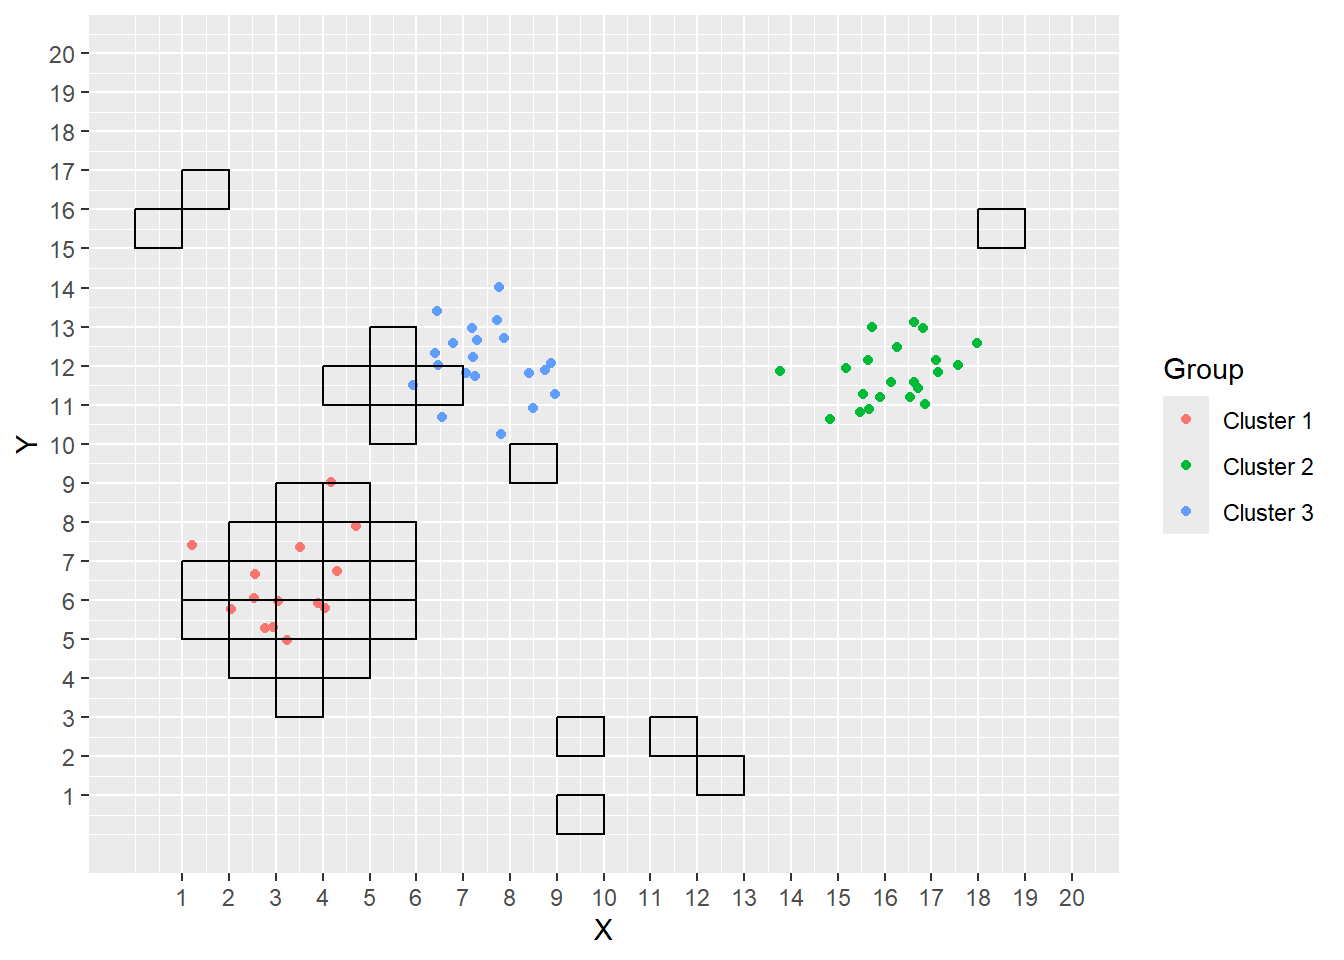
\includegraphics{Creating-the-framework_files/figure-latex/unnamed-chunk-9-1.pdf}

\subsubsection{Multiple samples from the same population of
points}\label{multiple-samples-from-the-same-population-of-points}

Goals: - take m samples from a population - return output in the same
format as \texttt{simulate\_one} but since there are m samples there
will be a list of lists

\begin{Shaded}
\begin{Highlighting}[]
\CommentTok{\# m numer of samples from the same population}
\NormalTok{simulate\_m}\OtherTok{\textless{}{-}}\ControlFlowTok{function}\NormalTok{(}\AttributeTok{m=}\DecValTok{10}\NormalTok{,}\AttributeTok{nclusters=}\DecValTok{3}\NormalTok{, }\AttributeTok{grid\_size=}\DecValTok{20}\NormalTok{,}\AttributeTok{n1=}\DecValTok{10}\NormalTok{,}\AttributeTok{force\_inclusion=}\ConstantTok{FALSE}\NormalTok{, }\AttributeTok{hard\_border=}\ConstantTok{TRUE}\NormalTok{,...  )\{}
\NormalTok{  results}\OtherTok{\textless{}{-}}\FunctionTok{list}\NormalTok{()}
  \CommentTok{\# generate clusters}
\NormalTok{  points}\OtherTok{\textless{}{-}}\FunctionTok{make\_clusters}\NormalTok{(}\AttributeTok{force\_inclusion =}\NormalTok{ force\_inclusion)}
  \ControlFlowTok{for}\NormalTok{(i }\ControlFlowTok{in} \DecValTok{1}\SpecialCharTok{:}\NormalTok{m)\{ }\CommentTok{\# loop for the m samples}
    \CommentTok{\# this is just the code from simulate\_one() see that for more comments}
\NormalTok{    sample\_tiles}\OtherTok{\textless{}{-}}\FunctionTok{get\_tiles}\NormalTok{(}\AttributeTok{n1=}\DecValTok{10}\NormalTok{,...)}
\NormalTok{    temp}\OtherTok{\textless{}{-}}\NormalTok{sample\_tiles}
\NormalTok{    occupied}\OtherTok{\textless{}{-}}\FunctionTok{apply}\NormalTok{(sample\_tiles,}\DecValTok{1}\NormalTok{,}\ControlFlowTok{function}\NormalTok{(x) }\FunctionTok{is\_occupied}\NormalTok{(x,points))}
    
\NormalTok{    neighbours}\OtherTok{\textless{}{-}}\FunctionTok{apply}\NormalTok{(sample\_tiles[occupied,], }\DecValTok{1}\NormalTok{, }\ControlFlowTok{function}\NormalTok{(x) }\FunctionTok{get\_neighbours}\NormalTok{(x,}\AttributeTok{hard\_border =}\NormalTok{ hard\_border))}\SpecialCharTok{\%\textgreater{}\%} \CommentTok{\# get neighbours}
      \FunctionTok{bind\_rows}\NormalTok{() }\SpecialCharTok{\%\textgreater{}\%} 
      \FunctionTok{as.data.frame}\NormalTok{() }
    
\NormalTok{    sample\_tiles}\OtherTok{\textless{}{-}}\FunctionTok{rbind}\NormalTok{(sample\_tiles,neighbours) }\SpecialCharTok{\%\textgreater{}\%}
      \FunctionTok{unique}\NormalTok{()}
     \CommentTok{\# keep looping until sample\_tiles does not grow}
    \ControlFlowTok{while}\NormalTok{(}\FunctionTok{dim}\NormalTok{(temp)[}\DecValTok{1}\NormalTok{]}\SpecialCharTok{!=}\FunctionTok{dim}\NormalTok{(sample\_tiles)[}\DecValTok{1}\NormalTok{])\{ }
      \CommentTok{\# save a copy to check against for updates}
\NormalTok{      temp}\OtherTok{\textless{}{-}}\NormalTok{sample\_tiles}
      \CommentTok{\# check whether or not they are occupied based on the clusters}
\NormalTok{      occupied}\OtherTok{\textless{}{-}}\FunctionTok{apply}\NormalTok{(sample\_tiles,}\DecValTok{1}\NormalTok{,}\ControlFlowTok{function}\NormalTok{(x) }\FunctionTok{is\_occupied}\NormalTok{(x,points))}
      \CommentTok{\# find the neighbours of the occupied points}
\NormalTok{      neighbours}\OtherTok{\textless{}{-}}\FunctionTok{apply}\NormalTok{(sample\_tiles[occupied,], }\DecValTok{1}\NormalTok{, }\ControlFlowTok{function}\NormalTok{(x)}\FunctionTok{get\_neighbours}\NormalTok{(x,}\AttributeTok{hard\_border =}\NormalTok{ hard\_border))}\SpecialCharTok{\%\textgreater{}\%} \CommentTok{\# get neighbours}
        \FunctionTok{bind\_rows}\NormalTok{() }\SpecialCharTok{\%\textgreater{}\%} \CommentTok{\# turn list of neighbours into tibble}
        \FunctionTok{as.data.frame}\NormalTok{() }\CommentTok{\# into dataframe}
      \CommentTok{\# update sample tiles to include neighbours}
\NormalTok{      sample\_tiles}\OtherTok{\textless{}{-}}\NormalTok{sample\_tiles }\SpecialCharTok{\%\textgreater{}\%}
        \FunctionTok{bind\_rows}\NormalTok{(neighbours) }\SpecialCharTok{\%\textgreater{}\%}
        \FunctionTok{unique}\NormalTok{()}
\NormalTok{    \}}
    
    \CommentTok{\# get the values of the response for each unit in the sample}
\NormalTok{    sample\_tiles}\SpecialCharTok{$}\NormalTok{y\_k}\OtherTok{\textless{}{-}}\FunctionTok{apply}\NormalTok{(sample\_tiles,}\DecValTok{1}\NormalTok{,}\ControlFlowTok{function}\NormalTok{(x) }\FunctionTok{tile\_sum}\NormalTok{(x, points))}
    \CommentTok{\# get the number of units in each network m\_k and add occupied to sample\_tiles}
\NormalTok{    sample\_tiles}\OtherTok{\textless{}{-}}\NormalTok{sample\_tiles}\SpecialCharTok{\%\textgreater{}\%}
      \FunctionTok{cbind}\NormalTok{(occupied)}\SpecialCharTok{\%\textgreater{}\%}
      \FunctionTok{group\_by}\NormalTok{(k)}\SpecialCharTok{\%\textgreater{}\%}
      \FunctionTok{mutate}\NormalTok{(}\AttributeTok{m\_k=}\FunctionTok{sum}\NormalTok{(occupied))}
    \CommentTok{\# minimum for m\_k is 1 not 0, set all 0s to 1}
\NormalTok{    sample\_tiles}\SpecialCharTok{$}\NormalTok{m\_k[sample\_tiles}\SpecialCharTok{$}\NormalTok{m\_k}\SpecialCharTok{==}\DecValTok{0}\NormalTok{]}\OtherTok{\textless{}{-}}\DecValTok{1}
    
\NormalTok{    results[[i]]}\OtherTok{\textless{}{-}}\FunctionTok{list}\NormalTok{(}\AttributeTok{sample\_tiles=}\NormalTok{sample\_tiles,}
                                  \AttributeTok{points=}\NormalTok{points,}
                                  \AttributeTok{nclusters=}\NormalTok{nclusters,}
                                  \AttributeTok{grid\_size=}\NormalTok{grid\_size,}
                                  \AttributeTok{n1=}\NormalTok{n1)}
\NormalTok{  \}}
  \FunctionTok{return}\NormalTok{(results)}
\NormalTok{\}}

\FunctionTok{set.seed}\NormalTok{(pi)}
\NormalTok{sim\_data\_m}\OtherTok{\textless{}{-}}\FunctionTok{simulate\_m}\NormalTok{()}
\end{Highlighting}
\end{Shaded}

When trying to write this simulation the largest issue I ran in to was
determining how to treat points that lie outside of the grid. Should
they be included in the sample? should they be ignored? should I change
the generating mechanism to force points to be bounded by the edges?
There are lots of things you need to specify in regards to how the
points are generated. This seems like it could also be an issue that
comes up in practical situations as well, for example the case where you
have a defined area you are allowed to collect samples from but the
thing you are measuring can occur up to and outside of that area. It
seems like we would be underestimating the average number in the greater
population if those are excluded from the cluster since it means we are
underestimating the cluster size.

\section{Finding the HT and HH
Estimators}\label{finding-the-ht-and-hh-estimators}

\subsection{Vocabulary}\label{vocabulary}

\begin{itemize}
\tightlist
\item
  neighborhood: the collection of units that are immediately included in
  the sample if a given unit is included. This relationship is symmetric
  and is typically (but not necessarily) geographic.
\item
  Cluster: the collection of all the units that are observed under the
  design as a result of initial selection of unit \(i\)
\item
  Network: selection of any unit within the network would lead to the
  inclusion in the sample of every other unit in the network.
\item
  edge unit: any unit not satisfying the condition but in the
  neighborhood of one that does
\end{itemize}

\subsection{Hansen-Hurwitz}\label{hansen-hurwitz}

\begin{itemize}
\tightlist
\item
  Let \(\Psi_k\) be the network that includes unit \(k\) and \(m_k\) be
  the number of units in that network. Any unit not satisfying the
  criterion is size \(1\).
\item
  Let \(\bar y_k^*=(m_k)^{-1}\sum_{j\in\Psi_k}y_j\) represent the
  average number of observations in the network that includes the
  \(k\)th unit of the initial sample
\item
  The modified Hansen-Hurwitz estimators given as
  \(t_{HH^*}=n_1^{-1}\sum^{n_1}_{k=1}\bar y_k^*\)
\end{itemize}

\subsubsection{Steps}\label{steps}

\begin{itemize}
\tightlist
\item
  Find average number of response in each network

  \begin{itemize}
  \tightlist
  \item
    file the average number of the response in a single tile.
  \end{itemize}
\item
  compute estimator using the averages
\end{itemize}

\paragraph{Applying the function to a single
sample}\label{applying-the-function-to-a-single-sample}

\begin{Shaded}
\begin{Highlighting}[]
\NormalTok{modified\_HH}\OtherTok{\textless{}{-}}\ControlFlowTok{function}\NormalTok{(sim\_data,}\AttributeTok{plot=}\NormalTok{F,}\AttributeTok{n1=}\DecValTok{10}\NormalTok{,...)\{}
  \CommentTok{\# Find the hansen hurwitz estimator of a sample called sim\_data}
  \ControlFlowTok{if}\NormalTok{(plot}\SpecialCharTok{==}\NormalTok{T)\{ }\CommentTok{\# plot sample}
    \FunctionTok{plot\_clusters}\NormalTok{(sim\_data}\SpecialCharTok{$}\NormalTok{points,}\AttributeTok{samp=}\NormalTok{sim\_data}\SpecialCharTok{$}\NormalTok{sample\_tiles)}
\NormalTok{  \}}
  
  \CommentTok{\# sample\_one$points and sample\_one$sample\_tiles}
  \CommentTok{\# get the response values for each tile sampled}
\NormalTok{  y\_k}\OtherTok{\textless{}{-}}\NormalTok{sim\_data}\SpecialCharTok{$}\NormalTok{sample\_tiles}\SpecialCharTok{$}\NormalTok{y\_k}
  \CommentTok{\# find the sum of each network that a unit belongs to this returns}
  \CommentTok{\# k and the mean}
\NormalTok{  temp}\OtherTok{\textless{}{-}}\FunctionTok{data.frame}\NormalTok{(y\_k,}\AttributeTok{group=}\NormalTok{sim\_data}\SpecialCharTok{$}\NormalTok{sample\_tiles}\SpecialCharTok{$}\NormalTok{k) }\SpecialCharTok{\%\textgreater{}\%}
    \FunctionTok{group\_by}\NormalTok{(group)}\SpecialCharTok{\%\textgreater{}\%}
    \FunctionTok{filter}\NormalTok{(y\_k}\SpecialCharTok{\textgreater{}}\DecValTok{0}\NormalTok{) }\SpecialCharTok{\%\textgreater{}\%}
    \FunctionTok{summarize}\NormalTok{(}\AttributeTok{network\_means=}\FunctionTok{mean}\NormalTok{(y\_k))}
  
\NormalTok{  means}\OtherTok{\textless{}{-}}\FunctionTok{data.frame}\NormalTok{(}\AttributeTok{init\_sample=}\DecValTok{1}\SpecialCharTok{:}\NormalTok{n1,}\AttributeTok{network\_means=}\FunctionTok{rep}\NormalTok{(}\DecValTok{0}\NormalTok{,n1))}
\NormalTok{  means[temp}\SpecialCharTok{$}\NormalTok{group,}\DecValTok{2}\NormalTok{]}\OtherTok{\textless{}{-}}\NormalTok{temp}\SpecialCharTok{$}\NormalTok{network\_means}
  \FunctionTok{mean}\NormalTok{(means}\SpecialCharTok{$}\NormalTok{network\_means)}
\NormalTok{\}}

\FunctionTok{modified\_HH}\NormalTok{(sim\_data,}\AttributeTok{plot=}\NormalTok{T)}
\end{Highlighting}
\end{Shaded}

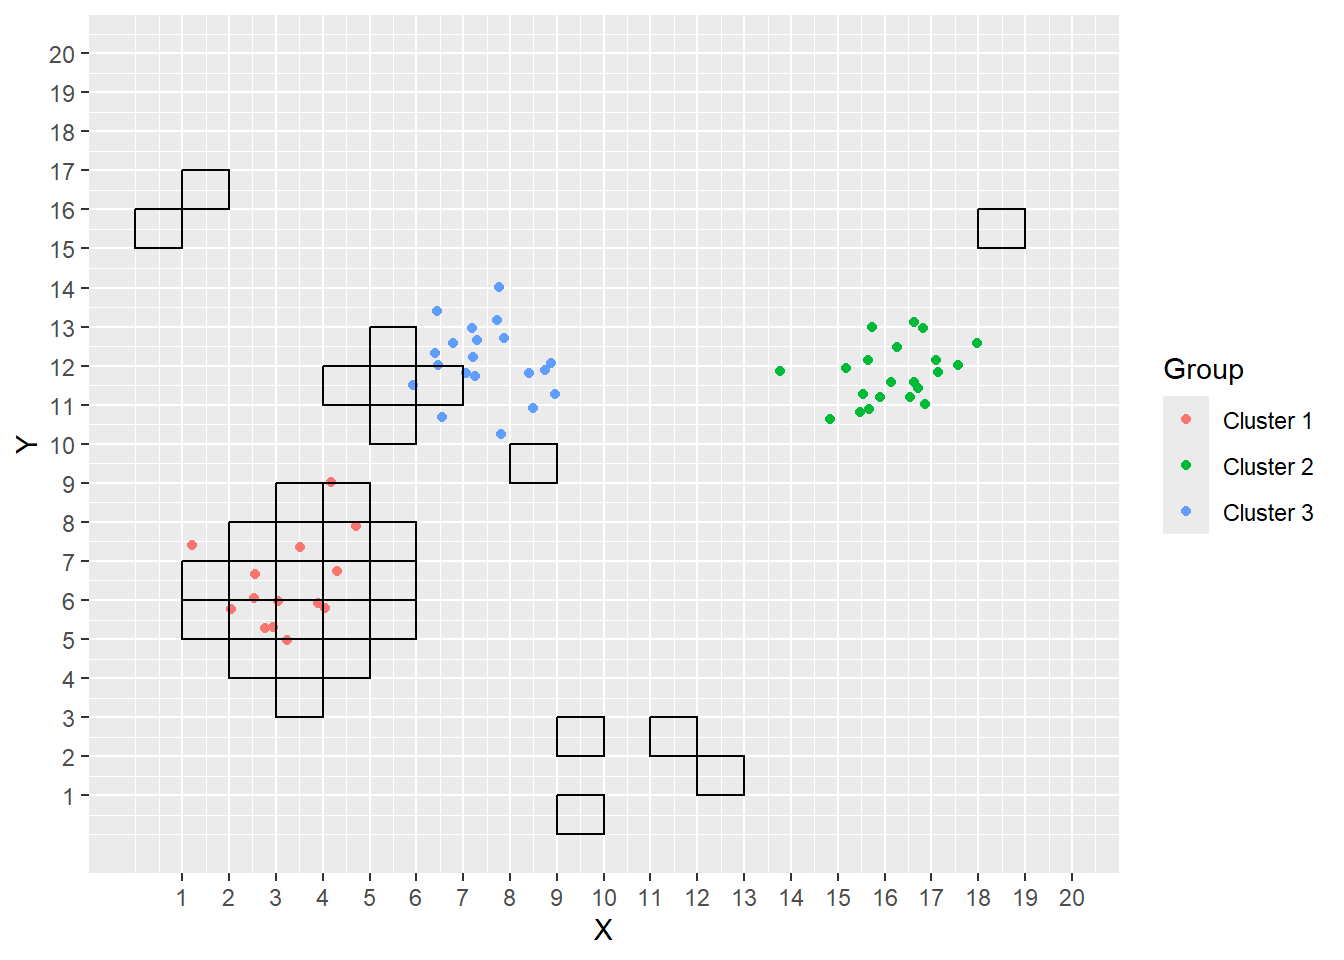
\includegraphics{Creating-the-framework_files/figure-latex/unnamed-chunk-11-1.pdf}

\begin{verbatim}
## [1] 0.25
\end{verbatim}

\subsection{Hovritz-Thompson}\label{hovritz-thompson}

The classic Horvitz-Thompson estimator is given by dividing each y-value
by the associated inclusion probability and is an unbiased estimator of
the population mean. This is not viable in adaptive cluster sampling as
the inclusion probabilities for all units are not known. None-the-less
we can still create an unbiased estimator by modifying the
Horvitz-Thompson estimator. First we define
\[\alpha^*_k=1-{N-m_k\choose n_1}/{N\choose n_1}\] Where \(m_k\) is the
number of units in the network that includes unit \(k\), \(N\) is the
number of units in the population, and \(n_1\) is the number of units in
the initial sample. Next let
\[J_k=\begin{cases}0& \text{If the condition is not satisfied} \\ 1 & \text{Otherwise}\end{cases}\]
Then the modified estimator is given by
\[t_{{HT}^*}=N^{-1}\sum^v_{k=1}y_kJ_k/\alpha^*_k\] where \(v\) is the
number of distinct units in the sample

\subsubsection{Steps}\label{steps-1}

\begin{itemize}
\tightlist
\item
  Find \(\alpha^*_k\) for each unit in the sample
\item
  Find \(y_kJ_k/\alpha^*_k\) for each unit
\item
  Find \(t_{HT^*}\)
\end{itemize}

\paragraph{\texorpdfstring{\(\alpha^*_k\)}{\textbackslash alpha\^{}*\_k}}\label{alpha_k}

\[\alpha^*_k=1-{N-m_k\choose n_1}/{N\choose n_1}\]

\begin{Shaded}
\begin{Highlighting}[]
\NormalTok{alpha\_k}\OtherTok{\textless{}{-}}\ControlFlowTok{function}\NormalTok{(sim\_data)\{}
  \CommentTok{\# get the response values for each tile sampled}
\NormalTok{  y\_k}\OtherTok{\textless{}{-}}\NormalTok{sim\_data}\SpecialCharTok{$}\NormalTok{sample\_tiles}\SpecialCharTok{$}\NormalTok{y\_k}
\NormalTok{  n1}\OtherTok{\textless{}{-}}\NormalTok{sim\_data}\SpecialCharTok{$}\NormalTok{n1}
\NormalTok{  N}\OtherTok{\textless{}{-}}\NormalTok{sim\_data}\SpecialCharTok{$}\NormalTok{grid\_size}\SpecialCharTok{\^{}}\DecValTok{2}
  \DecValTok{1}\SpecialCharTok{{-}}\FunctionTok{choose}\NormalTok{(N}\SpecialCharTok{{-}}\NormalTok{sim\_data}\SpecialCharTok{$}\NormalTok{sample\_tiles}\SpecialCharTok{$}\NormalTok{m\_k, sim\_data}\SpecialCharTok{$}\NormalTok{n1)}\SpecialCharTok{/}\FunctionTok{choose}\NormalTok{(N,sim\_data}\SpecialCharTok{$}\NormalTok{n1)}
\NormalTok{\}}
\FunctionTok{alpha\_k}\NormalTok{(sim\_data)}
\end{Highlighting}
\end{Shaded}

\begin{verbatim}
##  [1] 0.0250000 0.0250000 0.0250000 0.0250000 0.0250000 0.1848315 0.0250000
##  [8] 0.0250000 0.0250000 0.0250000 0.0250000 0.0250000 0.0250000 0.0250000
## [15] 0.1848315 0.1848315 0.1848315 0.1848315 0.1848315 0.1848315 0.1848315
## [22] 0.1848315 0.1848315 0.1848315 0.1848315 0.1848315 0.1848315 0.1848315
## [29] 0.1848315 0.1848315 0.1848315 0.1848315 0.1848315
\end{verbatim}

\paragraph{Finding the estimator}\label{finding-the-estimator}

\[t_{{HT}^*}=N^{-1}\sum^v_{k=1}y_kJ_k/\alpha^*_k\]

\begin{Shaded}
\begin{Highlighting}[]
\NormalTok{modified\_TH}\OtherTok{\textless{}{-}}\ControlFlowTok{function}\NormalTok{(sim\_data,}\AttributeTok{plot=}\NormalTok{F)\{}
  \ControlFlowTok{if}\NormalTok{(plot}\SpecialCharTok{==}\NormalTok{T)\{}
    \FunctionTok{plot\_clusters}\NormalTok{(sim\_data}\SpecialCharTok{$}\NormalTok{points,}\AttributeTok{samp=}\NormalTok{sim\_data}\SpecialCharTok{$}\NormalTok{sample\_tiles)}
\NormalTok{  \}}
\NormalTok{  a\_k}\OtherTok{\textless{}{-}}\FunctionTok{alpha\_k}\NormalTok{(sim\_data)}
\NormalTok{  N}\OtherTok{\textless{}{-}}\NormalTok{sim\_data}\SpecialCharTok{$}\NormalTok{grid\_size}\SpecialCharTok{\^{}}\DecValTok{2}
\NormalTok{  y\_k}\OtherTok{\textless{}{-}}\NormalTok{sim\_data}\SpecialCharTok{$}\NormalTok{sample\_tiles}\SpecialCharTok{$}\NormalTok{y\_k}
\NormalTok{  J\_k}\OtherTok{\textless{}{-}}\NormalTok{sim\_data}\SpecialCharTok{$}\NormalTok{sample\_tiles}\SpecialCharTok{$}\NormalTok{occupied}
  \DecValTok{1}\SpecialCharTok{/}\NormalTok{N}\SpecialCharTok{*}\FunctionTok{sum}\NormalTok{(y\_k}\SpecialCharTok{*}\NormalTok{J\_k}\SpecialCharTok{/}\NormalTok{a\_k)}
\NormalTok{\}}

\FunctionTok{modified\_TH}\NormalTok{(sim\_data)}
\end{Highlighting}
\end{Shaded}

\begin{verbatim}
## [1] 0.26231
\end{verbatim}

\section{Running simulations}\label{running-simulations}

\subsection{Initial results, Hard border, inclusion not
forced}\label{initial-results-hard-border-inclusion-not-forced}

This was the first simulation performed where 1000 populations were
sampled once, this limits what we are able to see though as the
variation of the sampling method for a given population may also be of
interest. Moving forward with simulations rather than sampling thousands
of populations we will only generate 9 populations but sample from them
1000 times each.

\begin{Shaded}
\begin{Highlighting}[]
\NormalTok{n\_sim}\OtherTok{\textless{}{-}}\DecValTok{1000}
\NormalTok{results}\OtherTok{\textless{}{-}}\FunctionTok{data.frame}\NormalTok{(}\AttributeTok{HH=}\FunctionTok{rep}\NormalTok{(}\ConstantTok{NA}\NormalTok{,n\_sim),}
                    \AttributeTok{TH=}\FunctionTok{rep}\NormalTok{(}\ConstantTok{NA}\NormalTok{,n\_sim),}
                    \AttributeTok{Truth=}\FunctionTok{rep}\NormalTok{(}\ConstantTok{NA}\NormalTok{,n\_sim))}
\ControlFlowTok{for}\NormalTok{(i }\ControlFlowTok{in} \DecValTok{1}\SpecialCharTok{:}\NormalTok{n\_sim)\{}
\NormalTok{  sim\_data}\OtherTok{\textless{}{-}}\FunctionTok{simulate\_one}\NormalTok{()}
\NormalTok{  results}\SpecialCharTok{$}\NormalTok{HH[i]}\OtherTok{\textless{}{-}}\FunctionTok{modified\_HH}\NormalTok{(sim\_data)}
\NormalTok{  results}\SpecialCharTok{$}\NormalTok{TH[i]}\OtherTok{\textless{}{-}}\FunctionTok{modified\_TH}\NormalTok{(sim\_data)}
\NormalTok{  results}\SpecialCharTok{$}\NormalTok{Truth[i]}\OtherTok{\textless{}{-}}\FunctionTok{length}\NormalTok{(sim\_data}\SpecialCharTok{$}\NormalTok{points}\SpecialCharTok{$}\NormalTok{X)}\SpecialCharTok{/}\NormalTok{(sim\_data}\SpecialCharTok{$}\NormalTok{grid\_size}\SpecialCharTok{\^{}}\DecValTok{2}\NormalTok{)}
\NormalTok{\}}
\FunctionTok{write.csv}\NormalTok{(results,}\AttributeTok{file=}\StringTok{"sampling 1000 populations.csv"}\NormalTok{)}
\end{Highlighting}
\end{Shaded}

\begin{Shaded}
\begin{Highlighting}[]
\NormalTok{results}\OtherTok{\textless{}{-}}\FunctionTok{read\_csv}\NormalTok{(}\StringTok{"sampling 1000 populations.csv"}\NormalTok{,}\AttributeTok{show\_col\_types =} \ConstantTok{FALSE}\NormalTok{)}
\end{Highlighting}
\end{Shaded}

\begin{verbatim}
## New names:
## * `` -> `...1`
\end{verbatim}

\begin{Shaded}
\begin{Highlighting}[]
\NormalTok{results\_long}\OtherTok{\textless{}{-}}\NormalTok{results }\SpecialCharTok{\%\textgreater{}\%} 
  \FunctionTok{pivot\_longer}\NormalTok{(}\AttributeTok{cols =}\NormalTok{ HH}\SpecialCharTok{:}\NormalTok{Truth,}
               \AttributeTok{names\_to =} \StringTok{"Estimator"}\NormalTok{, }
               \AttributeTok{values\_to =} \StringTok{"Value"}\NormalTok{)}

\FunctionTok{ggplot}\NormalTok{(results\_long,}\FunctionTok{aes}\NormalTok{(}\AttributeTok{x=}\NormalTok{Value, }\AttributeTok{y=}\NormalTok{Estimator, }\AttributeTok{fill=}\NormalTok{Estimator))}\SpecialCharTok{+}
  \FunctionTok{geom\_density\_ridges}\NormalTok{(}\AttributeTok{alpha=}\FloatTok{0.6}\NormalTok{, }\AttributeTok{stat=}\StringTok{"binline"}\NormalTok{,}\AttributeTok{bins=}\DecValTok{20}\NormalTok{,}\AttributeTok{scale=}\DecValTok{1}\NormalTok{)}\SpecialCharTok{+}
  \FunctionTok{theme\_ridges}\NormalTok{()}\SpecialCharTok{+}
  \FunctionTok{theme}\NormalTok{(}\AttributeTok{legend.position=}\StringTok{"none"}\NormalTok{,}
        \AttributeTok{axis.title.y =} \FunctionTok{element\_text}\NormalTok{( }\AttributeTok{hjust =} \FloatTok{0.5}\NormalTok{),}
        \AttributeTok{axis.title.x =} \FunctionTok{element\_text}\NormalTok{( }\AttributeTok{hjust =} \FloatTok{0.5}\NormalTok{))}\SpecialCharTok{+}
  \FunctionTok{xlab}\NormalTok{(}\StringTok{"Estimate"}\NormalTok{) }\SpecialCharTok{+}
  \FunctionTok{ylab}\NormalTok{(}\StringTok{"Frequency"}\NormalTok{)}\SpecialCharTok{+}
  \FunctionTok{ggtitle}\NormalTok{(}\StringTok{"Are adaptive cluster sampling estimators reliable?"}\NormalTok{)}\SpecialCharTok{+}
  \FunctionTok{scale\_fill\_manual}\NormalTok{(}\AttributeTok{values=}\FunctionTok{c}\NormalTok{(}\StringTok{"lightblue3"}\NormalTok{,}\StringTok{"lightblue3"}\NormalTok{,}\StringTok{"red3"}\NormalTok{))}
\end{Highlighting}
\end{Shaded}

\includegraphics{Creating-the-framework_files/figure-latex/unnamed-chunk-15-1.pdf}
\#\# exploring combinations of inclusion and border type Below are
simulations for all four combinations of border type and inclusion type
for 9 populations. There are 4 loops for simulations, one for inclusion
type, one for border type, one for the 9 populations, and one to compute
the estimators of the 1000 samples for the 9 populations.

\begin{Shaded}
\begin{Highlighting}[]
\NormalTok{m\_samples}\OtherTok{\textless{}{-}}\DecValTok{1000} \CommentTok{\#}
\NormalTok{n\_pops}\OtherTok{\textless{}{-}}\DecValTok{9}
\NormalTok{border\_type}\OtherTok{\textless{}{-}}\FunctionTok{c}\NormalTok{(}\ConstantTok{FALSE}\NormalTok{,}\ConstantTok{TRUE}\NormalTok{) }\CommentTok{\# h}
\NormalTok{border\_label}\OtherTok{\textless{}{-}}\FunctionTok{c}\NormalTok{(}\StringTok{"hard"}\NormalTok{,}\StringTok{"soft"}\NormalTok{)}
\NormalTok{inclusion\_type}\OtherTok{\textless{}{-}}\FunctionTok{c}\NormalTok{(}\ConstantTok{FALSE}\NormalTok{,}\ConstantTok{TRUE}\NormalTok{) }\CommentTok{\# k}
\NormalTok{inclusion\_label}\OtherTok{\textless{}{-}}\FunctionTok{c}\NormalTok{(}\StringTok{"not\_"}\NormalTok{,}\StringTok{""}\NormalTok{)}

\ControlFlowTok{for}\NormalTok{(h }\ControlFlowTok{in} \DecValTok{1}\SpecialCharTok{:}\FunctionTok{length}\NormalTok{(border\_type))\{}
  \ControlFlowTok{for}\NormalTok{(k }\ControlFlowTok{in} \DecValTok{1}\SpecialCharTok{:}\FunctionTok{length}\NormalTok{(inclusion\_type))\{}
    \CommentTok{\# Create blank dataframes for the estimates and the populations of points}
\NormalTok{    results}\OtherTok{\textless{}{-}}\FunctionTok{data.frame}\NormalTok{(}\AttributeTok{HH=}\FunctionTok{rep}\NormalTok{(}\ConstantTok{NA}\NormalTok{,n\_pops}\SpecialCharTok{*}\NormalTok{m\_samples),}
                        \AttributeTok{TH=}\FunctionTok{rep}\NormalTok{(}\ConstantTok{NA}\NormalTok{,n\_pops}\SpecialCharTok{*}\NormalTok{m\_samples),}
                        \AttributeTok{Truth=}\FunctionTok{rep}\NormalTok{(}\ConstantTok{NA}\NormalTok{,n\_pops}\SpecialCharTok{*}\NormalTok{m\_samples),}
                        \AttributeTok{Population=}\FunctionTok{rep}\NormalTok{(}\ConstantTok{NA}\NormalTok{,n\_pops}\SpecialCharTok{*}\NormalTok{m\_samples))}
    
\NormalTok{    population\_points}\OtherTok{\textless{}{-}}\FunctionTok{data.frame}\NormalTok{(}\AttributeTok{X=}\FunctionTok{c}\NormalTok{(),}\AttributeTok{Y=}\FunctionTok{c}\NormalTok{(),}\AttributeTok{Group=}\FunctionTok{c}\NormalTok{(),}\AttributeTok{Population=}\FunctionTok{c}\NormalTok{())}
    \CommentTok{\# set seed to ensure each set of populations are the same}
    \FunctionTok{set.seed}\NormalTok{(pi)}
    
    \ControlFlowTok{for}\NormalTok{(i }\ControlFlowTok{in} \DecValTok{1}\SpecialCharTok{:}\NormalTok{n\_pops)\{}
\NormalTok{      sim\_data}\OtherTok{\textless{}{-}}\FunctionTok{simulate\_m}\NormalTok{(}\AttributeTok{m=}\NormalTok{m\_samples,}
                           \AttributeTok{hard\_border =}\NormalTok{ border\_type[h], }
                           \AttributeTok{force\_inclusion =}\NormalTok{ inclusion\_type[k])}
      \CommentTok{\# save the population points to plot later}
\NormalTok{      population\_points}\OtherTok{\textless{}{-}}\NormalTok{population\_points}\SpecialCharTok{\%\textgreater{}\%}
        \FunctionTok{rbind}\NormalTok{( }\FunctionTok{cbind}\NormalTok{(sim\_data[[i]]}\SpecialCharTok{$}\NormalTok{points,}\AttributeTok{Population=}\FunctionTok{paste}\NormalTok{(}\StringTok{"pop"}\NormalTok{,i)) )}
      \ControlFlowTok{for}\NormalTok{(j }\ControlFlowTok{in} \DecValTok{1}\SpecialCharTok{:}\NormalTok{m\_samples)\{ }
        \CommentTok{\# for each sample from the population in sim\_data we compute our estimator}
        \CommentTok{\# saving estimators into results}
\NormalTok{        results}\SpecialCharTok{$}\NormalTok{HH[(i}\DecValTok{{-}1}\NormalTok{)}\SpecialCharTok{*}\NormalTok{m\_samples}\SpecialCharTok{+}\NormalTok{j]}\OtherTok{\textless{}{-}}\FunctionTok{modified\_HH}\NormalTok{(sim\_data[[j]])}
\NormalTok{        results}\SpecialCharTok{$}\NormalTok{TH[(i}\DecValTok{{-}1}\NormalTok{)}\SpecialCharTok{*}\NormalTok{m\_samples}\SpecialCharTok{+}\NormalTok{j]}\OtherTok{\textless{}{-}}\FunctionTok{modified\_TH}\NormalTok{(sim\_data[[j]])}
\NormalTok{        results}\SpecialCharTok{$}\NormalTok{Truth[(i}\DecValTok{{-}1}\NormalTok{)}\SpecialCharTok{*}\NormalTok{m\_samples}\SpecialCharTok{+}\NormalTok{j]}\OtherTok{\textless{}{-}}\FunctionTok{length}\NormalTok{(sim\_data[[j]]}\SpecialCharTok{$}\NormalTok{points}\SpecialCharTok{$}\NormalTok{X)}\SpecialCharTok{/}\NormalTok{(sim\_data[[j]]}\SpecialCharTok{$}\NormalTok{grid\_size}\SpecialCharTok{\^{}}\DecValTok{2}\NormalTok{)}
\NormalTok{        results}\SpecialCharTok{$}\NormalTok{Population[(i}\DecValTok{{-}1}\NormalTok{)}\SpecialCharTok{*}\NormalTok{m\_samples}\SpecialCharTok{+}\NormalTok{j]}\OtherTok{\textless{}{-}}\FunctionTok{paste}\NormalTok{(}\StringTok{"Population"}\NormalTok{,i)}
\NormalTok{      \}}
\NormalTok{    \}}
    
    \CommentTok{\# save end results of simulation}
    \FunctionTok{write.csv}\NormalTok{(results,}\AttributeTok{file=}\FunctionTok{paste}\NormalTok{(}\StringTok{"estimates{-}inclusion\_"}\NormalTok{,}
\NormalTok{                                 inclusion\_label[k],}
                                 \StringTok{"forced{-}"}\NormalTok{,}
\NormalTok{                                 border\_label[h], }\StringTok{"\_border.csv"}\NormalTok{,}
                                 \AttributeTok{sep=}\StringTok{""}\NormalTok{))}
    \FunctionTok{write.csv}\NormalTok{(population\_points,}\AttributeTok{file=}\FunctionTok{paste}\NormalTok{(}\StringTok{"pop\_points{-}inclusion\_"}\NormalTok{,}
\NormalTok{                                           inclusion\_label[k],}
                                           \StringTok{"forced{-}"}\NormalTok{,}
\NormalTok{                                           border\_label[h],}
                                           \StringTok{"\_border.csv"}\NormalTok{,}\AttributeTok{sep=}\StringTok{""}\NormalTok{))}

\NormalTok{  \}}
\NormalTok{\}}
\end{Highlighting}
\end{Shaded}

\subsection{plotting simulation results and
populations}\label{plotting-simulation-results-and-populations}

\begin{Shaded}
\begin{Highlighting}[]
\ControlFlowTok{for}\NormalTok{(i }\ControlFlowTok{in} \FunctionTok{c}\NormalTok{(}\StringTok{"soft"}\NormalTok{,}\StringTok{"hard"}\NormalTok{))\{}
  \ControlFlowTok{for}\NormalTok{(j }\ControlFlowTok{in} \FunctionTok{c}\NormalTok{(}\StringTok{"\_not"}\NormalTok{,}\StringTok{""}\NormalTok{))\{}
    \CommentTok{\# read in results from simulation above}
\NormalTok{    results}\OtherTok{\textless{}{-}}\FunctionTok{read\_csv}\NormalTok{(}\FunctionTok{paste}\NormalTok{(}\StringTok{"estimates{-}inclusion"}\NormalTok{,j,}\StringTok{"\_forced{-}"}\NormalTok{,i,}\StringTok{"\_border.csv"}\NormalTok{,}\AttributeTok{sep=}\StringTok{""}\NormalTok{),}
                      \AttributeTok{show\_col\_types =} \ConstantTok{FALSE}\NormalTok{,}
                      \AttributeTok{col\_select =}\NormalTok{ HH}\SpecialCharTok{:}\NormalTok{Population)}
\NormalTok{    results\_long}\OtherTok{\textless{}{-}}\NormalTok{results}\SpecialCharTok{\%\textgreater{}\%}
      \FunctionTok{pivot\_longer}\NormalTok{(}\AttributeTok{cols =}\NormalTok{ HH}\SpecialCharTok{:}\NormalTok{TH,}
                   \AttributeTok{names\_to =} \StringTok{"Estimator"}\NormalTok{, }
                   \AttributeTok{values\_to =} \StringTok{"Value"}\NormalTok{)}
        \CommentTok{\# plot the distributions of the estimators across the 9 populations}
\NormalTok{    p}\OtherTok{\textless{}{-}}\FunctionTok{ggplot}\NormalTok{(results\_long,}\FunctionTok{aes}\NormalTok{(}\AttributeTok{x=}\NormalTok{Value, }\AttributeTok{y=}\NormalTok{Estimator, }\AttributeTok{fill=}\NormalTok{Estimator))}\SpecialCharTok{+}
      \FunctionTok{geom\_density\_ridges}\NormalTok{(}\AttributeTok{alpha=}\FloatTok{0.6}\NormalTok{, }\AttributeTok{stat=}\StringTok{"binline"}\NormalTok{,}\AttributeTok{bins=}\DecValTok{20}\NormalTok{,}\AttributeTok{scale=}\DecValTok{1}\NormalTok{)}\SpecialCharTok{+}
      \FunctionTok{theme\_ridges}\NormalTok{()}\SpecialCharTok{+}
      \FunctionTok{theme}\NormalTok{(}\AttributeTok{legend.position=}\StringTok{"none"}\NormalTok{,}
            \AttributeTok{axis.title.y =} \FunctionTok{element\_text}\NormalTok{( }\AttributeTok{hjust =} \FloatTok{0.5}\NormalTok{),}
            \AttributeTok{axis.title.x =} \FunctionTok{element\_text}\NormalTok{( }\AttributeTok{hjust =} \FloatTok{0.5}\NormalTok{))}\SpecialCharTok{+}
      \FunctionTok{xlab}\NormalTok{(}\StringTok{"Estimate"}\NormalTok{) }\SpecialCharTok{+}
      \FunctionTok{ylab}\NormalTok{(}\StringTok{"Frequency"}\NormalTok{)}\SpecialCharTok{+}
      \FunctionTok{ggtitle}\NormalTok{(}\StringTok{"Are adaptive cluster sampling estimators reliable?"}\NormalTok{,}
              \AttributeTok{subtitle=}\FunctionTok{paste}\NormalTok{(}\StringTok{"Inclusion"}\NormalTok{,}\FunctionTok{gsub}\NormalTok{(}\StringTok{"\_"}\NormalTok{,}\StringTok{""}\NormalTok{,j),}\StringTok{"forced,"}\NormalTok{, i,}\StringTok{"border finding neighbours"}\NormalTok{))}\SpecialCharTok{+}
      \FunctionTok{scale\_fill\_manual}\NormalTok{(}\AttributeTok{values=}\FunctionTok{c}\NormalTok{(}\StringTok{"lightblue3"}\NormalTok{,}\StringTok{"lightblue3"}\NormalTok{))}\SpecialCharTok{+}
      \FunctionTok{facet\_wrap}\NormalTok{(}\SpecialCharTok{\textasciitilde{}}\NormalTok{Population)}\SpecialCharTok{+}
      \FunctionTok{geom\_vline}\NormalTok{(}\FunctionTok{aes}\NormalTok{(}\AttributeTok{xintercept=}\NormalTok{Truth),}\AttributeTok{color=}\StringTok{"red3"}\NormalTok{)}
    \FunctionTok{plot}\NormalTok{(p)}
\NormalTok{  \}}
\NormalTok{\}}
\end{Highlighting}
\end{Shaded}

\begin{verbatim}
## New names:
## New names:
## * `` -> `...1`
\end{verbatim}

\includegraphics{Creating-the-framework_files/figure-latex/unnamed-chunk-17-1.pdf}

\begin{verbatim}
## New names:
## * `` -> `...1`
\end{verbatim}

\includegraphics{Creating-the-framework_files/figure-latex/unnamed-chunk-17-2.pdf}

\begin{verbatim}
## New names:
## * `` -> `...1`
\end{verbatim}

\includegraphics{Creating-the-framework_files/figure-latex/unnamed-chunk-17-3.pdf}
\includegraphics{Creating-the-framework_files/figure-latex/unnamed-chunk-17-4.pdf}

\begin{Shaded}
\begin{Highlighting}[]
\ControlFlowTok{for}\NormalTok{(i }\ControlFlowTok{in} \FunctionTok{c}\NormalTok{(}\StringTok{"\_not"}\NormalTok{,}\StringTok{""}\NormalTok{))\{}
\NormalTok{  population\_points}\OtherTok{\textless{}{-}}\FunctionTok{read\_csv}\NormalTok{(}\FunctionTok{paste}\NormalTok{(}\StringTok{"pop\_points{-}inclusion"}\NormalTok{,i,}\StringTok{"\_forced{-}soft\_border.csv"}\NormalTok{,}\AttributeTok{sep=}\StringTok{""}\NormalTok{),}
                      \AttributeTok{show\_col\_types =} \ConstantTok{FALSE}\NormalTok{)}
  \CommentTok{\# plot the 9 populations}
\NormalTok{  p}\OtherTok{\textless{}{-}}\FunctionTok{ggplot}\NormalTok{(population\_points,}\FunctionTok{aes}\NormalTok{(}\AttributeTok{x=}\NormalTok{X,}\AttributeTok{y=}\NormalTok{Y,}\AttributeTok{color=}\NormalTok{Group))}\SpecialCharTok{+}
    \FunctionTok{geom\_point}\NormalTok{()}\SpecialCharTok{+}
    \FunctionTok{facet\_wrap}\NormalTok{(}\SpecialCharTok{\textasciitilde{}}\NormalTok{Population)}\SpecialCharTok{+}
    \FunctionTok{ggtitle}\NormalTok{(}\StringTok{"How do these estimators vary across populations?"}\NormalTok{,}
            \AttributeTok{subtitle=}\FunctionTok{paste}\NormalTok{(}\StringTok{"Inclusion"}\NormalTok{,}\FunctionTok{gsub}\NormalTok{(}\StringTok{"\_"}\NormalTok{,}\StringTok{""}\NormalTok{,i),}\StringTok{"forced"}\NormalTok{))}\SpecialCharTok{+}
    \FunctionTok{scale\_x\_continuous}\NormalTok{(}\AttributeTok{breaks =} \FunctionTok{seq}\NormalTok{(}\DecValTok{1}\NormalTok{, }\DecValTok{20}\NormalTok{, }\DecValTok{1}\NormalTok{)) }\SpecialCharTok{+}
    \FunctionTok{scale\_y\_continuous}\NormalTok{(}\AttributeTok{breaks =} \FunctionTok{seq}\NormalTok{(}\DecValTok{1}\NormalTok{, }\DecValTok{20}\NormalTok{, }\DecValTok{1}\NormalTok{))}\SpecialCharTok{+}
    \FunctionTok{geom\_hline}\NormalTok{(}\AttributeTok{yintercept=}\FunctionTok{c}\NormalTok{(}\DecValTok{0}\NormalTok{,}\DecValTok{20}\NormalTok{))}\SpecialCharTok{+}
    \FunctionTok{geom\_vline}\NormalTok{(}\AttributeTok{xintercept=}\FunctionTok{c}\NormalTok{(}\DecValTok{0}\NormalTok{,}\DecValTok{20}\NormalTok{))}\SpecialCharTok{+}
    \FunctionTok{guides}\NormalTok{(}\AttributeTok{color=}\StringTok{"none"}\NormalTok{)}
  
  \FunctionTok{plot}\NormalTok{(p)}
\NormalTok{\}}
\end{Highlighting}
\end{Shaded}

\begin{verbatim}
## New names:
## New names:
## * `` -> `...1`
\end{verbatim}

\includegraphics{Creating-the-framework_files/figure-latex/unnamed-chunk-17-5.pdf}
\includegraphics{Creating-the-framework_files/figure-latex/unnamed-chunk-17-6.pdf}

\subsection{Inclusion not forced}\label{inclusion-not-forced}

\subsubsection{Hard border when finding
neighbours}\label{hard-border-when-finding-neighbours}

\begin{Shaded}
\begin{Highlighting}[]
\FunctionTok{set.seed}\NormalTok{(pi)}
\NormalTok{n\_samples}\OtherTok{\textless{}{-}}\DecValTok{1000}
\NormalTok{n\_pops}\OtherTok{\textless{}{-}}\DecValTok{9}
\CommentTok{\# Create blank dataframes for the estimates and the populations of points}
\NormalTok{results}\OtherTok{\textless{}{-}}\FunctionTok{data.frame}\NormalTok{(}\AttributeTok{HH=}\FunctionTok{rep}\NormalTok{(}\ConstantTok{NA}\NormalTok{,n\_pops}\SpecialCharTok{*}\NormalTok{n\_samples),}
                    \AttributeTok{TH=}\FunctionTok{rep}\NormalTok{(}\ConstantTok{NA}\NormalTok{,n\_pops}\SpecialCharTok{*}\NormalTok{n\_samples),}
                    \AttributeTok{Truth=}\FunctionTok{rep}\NormalTok{(}\ConstantTok{NA}\NormalTok{,n\_pops}\SpecialCharTok{*}\NormalTok{n\_samples),}
                    \AttributeTok{Population=}\FunctionTok{rep}\NormalTok{(}\ConstantTok{NA}\NormalTok{,n\_pops}\SpecialCharTok{*}\NormalTok{n\_samples))}

\NormalTok{population\_points}\OtherTok{\textless{}{-}}\FunctionTok{data.frame}\NormalTok{(}\AttributeTok{X=}\FunctionTok{c}\NormalTok{(),}\AttributeTok{Y=}\FunctionTok{c}\NormalTok{(),}\AttributeTok{Group=}\FunctionTok{c}\NormalTok{(),}\AttributeTok{Population=}\FunctionTok{c}\NormalTok{())}

\ControlFlowTok{for}\NormalTok{(i }\ControlFlowTok{in} \DecValTok{1}\SpecialCharTok{:}\NormalTok{n\_pops)\{}
\NormalTok{  sim\_data}\OtherTok{\textless{}{-}}\FunctionTok{simulate\_m}\NormalTok{(}\AttributeTok{m=}\NormalTok{n\_samples,}\AttributeTok{hard\_border =} \ConstantTok{TRUE}\NormalTok{, }\AttributeTok{force\_inclusion =} \ConstantTok{FALSE}\NormalTok{)}
  \CommentTok{\# save the population points to plot later}
\NormalTok{  population\_points}\OtherTok{\textless{}{-}}\NormalTok{population\_points}\SpecialCharTok{\%\textgreater{}\%}
    \FunctionTok{rbind}\NormalTok{( }\FunctionTok{cbind}\NormalTok{(sim\_data[[i]]}\SpecialCharTok{$}\NormalTok{points,}\AttributeTok{Population=}\FunctionTok{paste}\NormalTok{(}\StringTok{"pop"}\NormalTok{,i)) )}
  \ControlFlowTok{for}\NormalTok{(j }\ControlFlowTok{in} \DecValTok{1}\SpecialCharTok{:}\NormalTok{n\_samples)\{}
    \CommentTok{\# saving estimators into results}
\NormalTok{    results}\SpecialCharTok{$}\NormalTok{HH[(i}\DecValTok{{-}1}\NormalTok{)}\SpecialCharTok{*}\NormalTok{n\_samples}\SpecialCharTok{+}\NormalTok{j]}\OtherTok{\textless{}{-}}\FunctionTok{modified\_HH}\NormalTok{(sim\_data[[j]])}
\NormalTok{    results}\SpecialCharTok{$}\NormalTok{TH[(i}\DecValTok{{-}1}\NormalTok{)}\SpecialCharTok{*}\NormalTok{n\_samples}\SpecialCharTok{+}\NormalTok{j]}\OtherTok{\textless{}{-}}\FunctionTok{modified\_TH}\NormalTok{(sim\_data[[j]])}
\NormalTok{    results}\SpecialCharTok{$}\NormalTok{Truth[(i}\DecValTok{{-}1}\NormalTok{)}\SpecialCharTok{*}\NormalTok{n\_samples}\SpecialCharTok{+}\NormalTok{j]}\OtherTok{\textless{}{-}}\FunctionTok{length}\NormalTok{(sim\_data[[j]]}\SpecialCharTok{$}\NormalTok{points}\SpecialCharTok{$}\NormalTok{X)}\SpecialCharTok{/}\NormalTok{(sim\_data[[j]]}\SpecialCharTok{$}\NormalTok{grid\_size}\SpecialCharTok{\^{}}\DecValTok{2}\NormalTok{)}
\NormalTok{    results}\SpecialCharTok{$}\NormalTok{Population[(i}\DecValTok{{-}1}\NormalTok{)}\SpecialCharTok{*}\NormalTok{n\_samples}\SpecialCharTok{+}\NormalTok{j]}\OtherTok{\textless{}{-}}\FunctionTok{paste}\NormalTok{(}\StringTok{"Population"}\NormalTok{,i)}
\NormalTok{  \}}
\NormalTok{\}}

\CommentTok{\# save end results of simulation}
\FunctionTok{write.csv}\NormalTok{(results,}\AttributeTok{file=}\StringTok{"estimates{-}inclusion\_not\_forced{-}hard\_border.csv"}\NormalTok{)}
\FunctionTok{write.csv}\NormalTok{(population\_points,}\AttributeTok{file=}\StringTok{"pop\_points{-}inclusion\_not\_forced{-}hard\_border.csv"}\NormalTok{)}
\end{Highlighting}
\end{Shaded}

\begin{Shaded}
\begin{Highlighting}[]
\CommentTok{\# read in results from simulation above}
\NormalTok{results}\OtherTok{\textless{}{-}}\FunctionTok{read\_csv}\NormalTok{(}\StringTok{"estimates{-}inclusion\_not\_forced{-}hard\_border.csv"}\NormalTok{,}\AttributeTok{show\_col\_types =} \ConstantTok{FALSE}\NormalTok{)}
\end{Highlighting}
\end{Shaded}

\begin{verbatim}
## New names:
## * `` -> `...1`
\end{verbatim}

\begin{Shaded}
\begin{Highlighting}[]
\NormalTok{results\_long}\OtherTok{\textless{}{-}}\NormalTok{results}\SpecialCharTok{\%\textgreater{}\%}
  \FunctionTok{pivot\_longer}\NormalTok{(}\AttributeTok{cols =}\NormalTok{ HH}\SpecialCharTok{:}\NormalTok{TH,}
               \AttributeTok{names\_to =} \StringTok{"Estimator"}\NormalTok{, }
               \AttributeTok{values\_to =} \StringTok{"Value"}\NormalTok{)}

\NormalTok{population\_points}\OtherTok{\textless{}{-}}\FunctionTok{read\_csv}\NormalTok{(}\StringTok{"pop\_points{-}inclusion\_not\_forced{-}hard\_border.csv"}\NormalTok{,}\AttributeTok{show\_col\_types =} \ConstantTok{FALSE}\NormalTok{)}
\end{Highlighting}
\end{Shaded}

\begin{verbatim}
## New names:
## * `` -> `...1`
\end{verbatim}

\begin{Shaded}
\begin{Highlighting}[]
\CommentTok{\# plot the distributions of the estimators across the 9 populations}
\FunctionTok{ggplot}\NormalTok{(results\_long,}\FunctionTok{aes}\NormalTok{(}\AttributeTok{x=}\NormalTok{Value, }\AttributeTok{y=}\NormalTok{Estimator, }\AttributeTok{fill=}\NormalTok{Estimator))}\SpecialCharTok{+}
  \FunctionTok{geom\_density\_ridges}\NormalTok{(}\AttributeTok{alpha=}\FloatTok{0.6}\NormalTok{, }\AttributeTok{stat=}\StringTok{"binline"}\NormalTok{,}\AttributeTok{bins=}\DecValTok{20}\NormalTok{,}\AttributeTok{scale=}\DecValTok{1}\NormalTok{)}\SpecialCharTok{+}
  \FunctionTok{theme\_ridges}\NormalTok{()}\SpecialCharTok{+}
  \FunctionTok{theme}\NormalTok{(}\AttributeTok{legend.position=}\StringTok{"none"}\NormalTok{,}
        \AttributeTok{axis.title.y =} \FunctionTok{element\_text}\NormalTok{( }\AttributeTok{hjust =} \FloatTok{0.5}\NormalTok{),}
        \AttributeTok{axis.title.x =} \FunctionTok{element\_text}\NormalTok{( }\AttributeTok{hjust =} \FloatTok{0.5}\NormalTok{))}\SpecialCharTok{+}
  \FunctionTok{xlab}\NormalTok{(}\StringTok{"Estimate"}\NormalTok{) }\SpecialCharTok{+}
  \FunctionTok{ylab}\NormalTok{(}\StringTok{"Frequency"}\NormalTok{)}\SpecialCharTok{+}
  \FunctionTok{ggtitle}\NormalTok{(}\StringTok{"Are adaptive cluster sampling estimators reliable?"}\NormalTok{,}
          \AttributeTok{subtitle=}\StringTok{"Inclusion not forced, hard border finding neighbours"}\NormalTok{)}\SpecialCharTok{+}
  \FunctionTok{scale\_fill\_manual}\NormalTok{(}\AttributeTok{values=}\FunctionTok{c}\NormalTok{(}\StringTok{"lightblue3"}\NormalTok{,}\StringTok{"lightblue3"}\NormalTok{))}\SpecialCharTok{+}
  \FunctionTok{facet\_wrap}\NormalTok{(}\SpecialCharTok{\textasciitilde{}}\NormalTok{Population)}\SpecialCharTok{+}
  \FunctionTok{geom\_vline}\NormalTok{(}\FunctionTok{aes}\NormalTok{(}\AttributeTok{xintercept=}\NormalTok{Truth),}\AttributeTok{color=}\StringTok{"red3"}\NormalTok{)}
\end{Highlighting}
\end{Shaded}

\includegraphics{Creating-the-framework_files/figure-latex/unnamed-chunk-19-1.pdf}

\begin{Shaded}
\begin{Highlighting}[]
\CommentTok{\# plot the 9 populations}
\FunctionTok{ggplot}\NormalTok{(population\_points,}\FunctionTok{aes}\NormalTok{(}\AttributeTok{x=}\NormalTok{X,}\AttributeTok{y=}\NormalTok{Y,}\AttributeTok{color=}\NormalTok{Group))}\SpecialCharTok{+}
  \FunctionTok{geom\_point}\NormalTok{()}\SpecialCharTok{+}
  \FunctionTok{facet\_wrap}\NormalTok{(}\SpecialCharTok{\textasciitilde{}}\NormalTok{Population)}\SpecialCharTok{+}
  \FunctionTok{ggtitle}\NormalTok{(}\StringTok{"How do these estimators vary across populations?"}\NormalTok{,}
          \AttributeTok{subtitle=}\StringTok{"Inclusion not forced, hard border finding neighbours"}\NormalTok{)}
\end{Highlighting}
\end{Shaded}

\includegraphics{Creating-the-framework_files/figure-latex/unnamed-chunk-19-2.pdf}

\subsubsection{Soft border when finding
neighbours}\label{soft-border-when-finding-neighbours}

\begin{Shaded}
\begin{Highlighting}[]
\FunctionTok{set.seed}\NormalTok{(pi)}
\NormalTok{n\_samples}\OtherTok{\textless{}{-}}\DecValTok{1000}
\NormalTok{n\_pops}\OtherTok{\textless{}{-}}\DecValTok{9}
\CommentTok{\# estimator results}
\NormalTok{results}\OtherTok{\textless{}{-}}\FunctionTok{data.frame}\NormalTok{(}\AttributeTok{HH=}\FunctionTok{rep}\NormalTok{(}\ConstantTok{NA}\NormalTok{,n\_pops}\SpecialCharTok{*}\NormalTok{n\_samples),}
                    \AttributeTok{TH=}\FunctionTok{rep}\NormalTok{(}\ConstantTok{NA}\NormalTok{,n\_pops}\SpecialCharTok{*}\NormalTok{n\_samples),}
                    \AttributeTok{Truth=}\FunctionTok{rep}\NormalTok{(}\ConstantTok{NA}\NormalTok{,n\_pops}\SpecialCharTok{*}\NormalTok{n\_samples),}
                    \AttributeTok{Population=}\FunctionTok{rep}\NormalTok{(}\ConstantTok{NA}\NormalTok{,n\_pops}\SpecialCharTok{*}\NormalTok{n\_samples))}
\CommentTok{\# saving the population sampled from}
\NormalTok{population\_points}\OtherTok{\textless{}{-}}\FunctionTok{data.frame}\NormalTok{(}\AttributeTok{X=}\FunctionTok{c}\NormalTok{(),}\AttributeTok{Y=}\FunctionTok{c}\NormalTok{(),}\AttributeTok{Group=}\FunctionTok{c}\NormalTok{(),}\AttributeTok{Population=}\FunctionTok{c}\NormalTok{())}

\ControlFlowTok{for}\NormalTok{(i }\ControlFlowTok{in} \DecValTok{1}\SpecialCharTok{:}\NormalTok{n\_pops)\{ }\CommentTok{\# generating the populations and samples}
\NormalTok{  sim\_data}\OtherTok{\textless{}{-}}\FunctionTok{simulate\_m}\NormalTok{(}\AttributeTok{m=}\NormalTok{n\_samples,}\AttributeTok{hard\_border =} \ConstantTok{FALSE}\NormalTok{, }\AttributeTok{force\_inclusion =} \ConstantTok{FALSE}\NormalTok{)}
  \CommentTok{\# save the population points to plot later}
\NormalTok{  population\_points}\OtherTok{\textless{}{-}}\NormalTok{population\_points}\SpecialCharTok{\%\textgreater{}\%}
    \FunctionTok{rbind}\NormalTok{( }\FunctionTok{cbind}\NormalTok{(sim\_data[[i]]}\SpecialCharTok{$}\NormalTok{points,}\AttributeTok{Population=}\FunctionTok{paste}\NormalTok{(}\StringTok{"pop"}\NormalTok{,i)) )}
  \ControlFlowTok{for}\NormalTok{(j }\ControlFlowTok{in} \DecValTok{1}\SpecialCharTok{:}\NormalTok{n\_samples)\{}
    \CommentTok{\# save estimates for each sample}
\NormalTok{    results}\SpecialCharTok{$}\NormalTok{HH[(i}\DecValTok{{-}1}\NormalTok{)}\SpecialCharTok{*}\NormalTok{n\_samples}\SpecialCharTok{+}\NormalTok{j]}\OtherTok{\textless{}{-}}\FunctionTok{modified\_HH}\NormalTok{(sim\_data[[j]])}
\NormalTok{    results}\SpecialCharTok{$}\NormalTok{TH[(i}\DecValTok{{-}1}\NormalTok{)}\SpecialCharTok{*}\NormalTok{n\_samples}\SpecialCharTok{+}\NormalTok{j]}\OtherTok{\textless{}{-}}\FunctionTok{modified\_TH}\NormalTok{(sim\_data[[j]])}
\NormalTok{    results}\SpecialCharTok{$}\NormalTok{Truth[(i}\DecValTok{{-}1}\NormalTok{)}\SpecialCharTok{*}\NormalTok{n\_samples}\SpecialCharTok{+}\NormalTok{j]}\OtherTok{\textless{}{-}}\FunctionTok{length}\NormalTok{(sim\_data[[j]]}\SpecialCharTok{$}\NormalTok{points}\SpecialCharTok{$}\NormalTok{X)}\SpecialCharTok{/}\NormalTok{(sim\_data[[j]]}\SpecialCharTok{$}\NormalTok{grid\_size}\SpecialCharTok{\^{}}\DecValTok{2}\NormalTok{)}
\NormalTok{    results}\SpecialCharTok{$}\NormalTok{Population[(i}\DecValTok{{-}1}\NormalTok{)}\SpecialCharTok{*}\NormalTok{n\_samples}\SpecialCharTok{+}\NormalTok{j]}\OtherTok{\textless{}{-}}\FunctionTok{paste}\NormalTok{(}\StringTok{"Population"}\NormalTok{,i)}
\NormalTok{  \}}
\NormalTok{\}}
\CommentTok{\# save estimates of the samples and the populations sampled from}
\FunctionTok{write.csv}\NormalTok{(results,}\AttributeTok{file=}\StringTok{"estimates{-}inclusion\_not\_forced{-}soft\_border.csv"}\NormalTok{)}
\FunctionTok{write.csv}\NormalTok{(population\_points,}\AttributeTok{file=}\StringTok{"pop\_points{-}inclusion\_not\_forced{-}soft\_border.csv"}\NormalTok{)}
\end{Highlighting}
\end{Shaded}

\begin{Shaded}
\begin{Highlighting}[]
\NormalTok{results}\OtherTok{\textless{}{-}}\FunctionTok{read\_csv}\NormalTok{(}\StringTok{"estimates{-}inclusion\_not\_forced{-}soft\_border.csv"}\NormalTok{,}\AttributeTok{show\_col\_types =} \ConstantTok{FALSE}\NormalTok{)}
\end{Highlighting}
\end{Shaded}

\begin{verbatim}
## New names:
## * `` -> `...1`
\end{verbatim}

\begin{Shaded}
\begin{Highlighting}[]
\NormalTok{results\_long}\OtherTok{\textless{}{-}}\NormalTok{results}\SpecialCharTok{\%\textgreater{}\%}
  \FunctionTok{pivot\_longer}\NormalTok{(}\AttributeTok{cols =}\NormalTok{ HH}\SpecialCharTok{:}\NormalTok{TH,}
               \AttributeTok{names\_to =} \StringTok{"Estimator"}\NormalTok{, }
               \AttributeTok{values\_to =} \StringTok{"Value"}\NormalTok{)}

\NormalTok{population\_points}\OtherTok{\textless{}{-}}\FunctionTok{read\_csv}\NormalTok{(}\StringTok{"pop\_points{-}inclusion\_not\_forced{-}soft\_border.csv"}\NormalTok{,}\AttributeTok{show\_col\_types =} \ConstantTok{FALSE}\NormalTok{)}
\end{Highlighting}
\end{Shaded}

\begin{verbatim}
## New names:
## * `` -> `...1`
\end{verbatim}

\begin{Shaded}
\begin{Highlighting}[]
\FunctionTok{ggplot}\NormalTok{(results\_long,}\FunctionTok{aes}\NormalTok{(}\AttributeTok{x=}\NormalTok{Value, }\AttributeTok{y=}\NormalTok{Estimator, }\AttributeTok{fill=}\NormalTok{Estimator))}\SpecialCharTok{+}
  \FunctionTok{geom\_density\_ridges}\NormalTok{(}\AttributeTok{alpha=}\FloatTok{0.6}\NormalTok{, }\AttributeTok{stat=}\StringTok{"binline"}\NormalTok{,}\AttributeTok{bins=}\DecValTok{20}\NormalTok{,}\AttributeTok{scale=}\DecValTok{1}\NormalTok{)}\SpecialCharTok{+}
  \FunctionTok{theme\_ridges}\NormalTok{()}\SpecialCharTok{+}
  \FunctionTok{theme}\NormalTok{(}\AttributeTok{legend.position=}\StringTok{"none"}\NormalTok{,}
        \AttributeTok{axis.title.y =} \FunctionTok{element\_text}\NormalTok{( }\AttributeTok{hjust =} \FloatTok{0.5}\NormalTok{),}
        \AttributeTok{axis.title.x =} \FunctionTok{element\_text}\NormalTok{( }\AttributeTok{hjust =} \FloatTok{0.5}\NormalTok{))}\SpecialCharTok{+}
  \FunctionTok{xlab}\NormalTok{(}\StringTok{"Estimate"}\NormalTok{) }\SpecialCharTok{+}
  \FunctionTok{ylab}\NormalTok{(}\StringTok{"Frequency"}\NormalTok{)}\SpecialCharTok{+}
  \FunctionTok{ggtitle}\NormalTok{(}\StringTok{"Are adaptive cluster sampling estimators reliable?"}\NormalTok{,}
          \AttributeTok{subtitle=}\StringTok{"Inclusion not forced, soft border finding neighbours"}\NormalTok{)}\SpecialCharTok{+}
  \FunctionTok{scale\_fill\_manual}\NormalTok{(}\AttributeTok{values=}\FunctionTok{c}\NormalTok{(}\StringTok{"lightblue3"}\NormalTok{,}\StringTok{"lightblue3"}\NormalTok{))}\SpecialCharTok{+}
  \FunctionTok{facet\_wrap}\NormalTok{(}\SpecialCharTok{\textasciitilde{}}\NormalTok{Population)}\SpecialCharTok{+}
  \FunctionTok{geom\_vline}\NormalTok{(}\FunctionTok{aes}\NormalTok{(}\AttributeTok{xintercept=}\NormalTok{Truth),}\AttributeTok{color=}\StringTok{"red3"}\NormalTok{)}
\end{Highlighting}
\end{Shaded}

\includegraphics{Creating-the-framework_files/figure-latex/unnamed-chunk-21-1.pdf}

\begin{Shaded}
\begin{Highlighting}[]
\FunctionTok{ggplot}\NormalTok{(population\_points,}\FunctionTok{aes}\NormalTok{(}\AttributeTok{x=}\NormalTok{X,}\AttributeTok{y=}\NormalTok{Y,}\AttributeTok{color=}\NormalTok{Group))}\SpecialCharTok{+}
  \FunctionTok{geom\_point}\NormalTok{()}\SpecialCharTok{+}
  \FunctionTok{facet\_wrap}\NormalTok{(}\SpecialCharTok{\textasciitilde{}}\NormalTok{Population)}\SpecialCharTok{+}
  \FunctionTok{ggtitle}\NormalTok{(}\StringTok{"How do these estimators vary across populations?"}\NormalTok{,}
          \AttributeTok{subtitle=}\StringTok{"Inclusion not forced, soft border finding neighbours"}\NormalTok{)}
\end{Highlighting}
\end{Shaded}

\includegraphics{Creating-the-framework_files/figure-latex/unnamed-chunk-21-2.pdf}

\subsection{Inclusion forced}\label{inclusion-forced}

\subsubsection{Hard border when finding
neighbours}\label{hard-border-when-finding-neighbours-1}

\begin{Shaded}
\begin{Highlighting}[]
\FunctionTok{set.seed}\NormalTok{(pi)}
\NormalTok{n\_samples}\OtherTok{\textless{}{-}}\DecValTok{1000}
\NormalTok{n\_pops}\OtherTok{\textless{}{-}}\DecValTok{9}
\CommentTok{\# Create blank dataframes for the estimates and the populations of points}
\NormalTok{results}\OtherTok{\textless{}{-}}\FunctionTok{data.frame}\NormalTok{(}\AttributeTok{HH=}\FunctionTok{rep}\NormalTok{(}\ConstantTok{NA}\NormalTok{,n\_pops}\SpecialCharTok{*}\NormalTok{n\_samples),}
                    \AttributeTok{TH=}\FunctionTok{rep}\NormalTok{(}\ConstantTok{NA}\NormalTok{,n\_pops}\SpecialCharTok{*}\NormalTok{n\_samples),}
                    \AttributeTok{Truth=}\FunctionTok{rep}\NormalTok{(}\ConstantTok{NA}\NormalTok{,n\_pops}\SpecialCharTok{*}\NormalTok{n\_samples),}
                    \AttributeTok{Population=}\FunctionTok{rep}\NormalTok{(}\ConstantTok{NA}\NormalTok{,n\_pops}\SpecialCharTok{*}\NormalTok{n\_samples))}

\NormalTok{population\_points}\OtherTok{\textless{}{-}}\FunctionTok{data.frame}\NormalTok{(}\AttributeTok{X=}\FunctionTok{c}\NormalTok{(),}\AttributeTok{Y=}\FunctionTok{c}\NormalTok{(),}\AttributeTok{Group=}\FunctionTok{c}\NormalTok{(),}\AttributeTok{Population=}\FunctionTok{c}\NormalTok{())}

\ControlFlowTok{for}\NormalTok{(i }\ControlFlowTok{in} \DecValTok{1}\SpecialCharTok{:}\NormalTok{n\_pops)\{}
\NormalTok{  sim\_data}\OtherTok{\textless{}{-}}\FunctionTok{simulate\_m}\NormalTok{(}\AttributeTok{m=}\NormalTok{n\_samples,}\AttributeTok{hard\_border =} \ConstantTok{TRUE}\NormalTok{, }\AttributeTok{force\_inclusion =} \ConstantTok{TRUE}\NormalTok{)}
  \CommentTok{\# save the population points to plot later}
\NormalTok{  population\_points}\OtherTok{\textless{}{-}}\NormalTok{population\_points}\SpecialCharTok{\%\textgreater{}\%}
    \FunctionTok{rbind}\NormalTok{( }\FunctionTok{cbind}\NormalTok{(sim\_data[[i]]}\SpecialCharTok{$}\NormalTok{points,}\AttributeTok{Population=}\FunctionTok{paste}\NormalTok{(}\StringTok{"pop"}\NormalTok{,i)) )}
  \ControlFlowTok{for}\NormalTok{(j }\ControlFlowTok{in} \DecValTok{1}\SpecialCharTok{:}\NormalTok{n\_samples)\{}
    \CommentTok{\# saving estimators into results}
\NormalTok{    results}\SpecialCharTok{$}\NormalTok{HH[(i}\DecValTok{{-}1}\NormalTok{)}\SpecialCharTok{*}\NormalTok{n\_samples}\SpecialCharTok{+}\NormalTok{j]}\OtherTok{\textless{}{-}}\FunctionTok{modified\_HH}\NormalTok{(sim\_data[[j]])}
\NormalTok{    results}\SpecialCharTok{$}\NormalTok{TH[(i}\DecValTok{{-}1}\NormalTok{)}\SpecialCharTok{*}\NormalTok{n\_samples}\SpecialCharTok{+}\NormalTok{j]}\OtherTok{\textless{}{-}}\FunctionTok{modified\_TH}\NormalTok{(sim\_data[[j]])}
\NormalTok{    results}\SpecialCharTok{$}\NormalTok{Truth[(i}\DecValTok{{-}1}\NormalTok{)}\SpecialCharTok{*}\NormalTok{n\_samples}\SpecialCharTok{+}\NormalTok{j]}\OtherTok{\textless{}{-}}\FunctionTok{length}\NormalTok{(sim\_data[[j]]}\SpecialCharTok{$}\NormalTok{points}\SpecialCharTok{$}\NormalTok{X)}\SpecialCharTok{/}\NormalTok{(sim\_data[[j]]}\SpecialCharTok{$}\NormalTok{grid\_size}\SpecialCharTok{\^{}}\DecValTok{2}\NormalTok{)}
\NormalTok{    results}\SpecialCharTok{$}\NormalTok{Population[(i}\DecValTok{{-}1}\NormalTok{)}\SpecialCharTok{*}\NormalTok{n\_samples}\SpecialCharTok{+}\NormalTok{j]}\OtherTok{\textless{}{-}}\FunctionTok{paste}\NormalTok{(}\StringTok{"Population"}\NormalTok{,i)}
\NormalTok{  \}}
\NormalTok{\}}

\CommentTok{\# save end results of simulation}
\FunctionTok{write.csv}\NormalTok{(results,}\AttributeTok{file=}\StringTok{"estimates{-}inclusion\_forced{-}hard\_border.csv"}\NormalTok{)}
\FunctionTok{write.csv}\NormalTok{(population\_points,}\AttributeTok{file=}\StringTok{"pop\_points{-}inclusion\_forced{-}hard\_border.csv"}\NormalTok{)}
\end{Highlighting}
\end{Shaded}

\begin{Shaded}
\begin{Highlighting}[]
\CommentTok{\# read in results from simulation above}
\NormalTok{results}\OtherTok{\textless{}{-}}\FunctionTok{read\_csv}\NormalTok{(}\StringTok{"estimates{-}inclusion\_forced{-}hard\_border.csv"}\NormalTok{,}\AttributeTok{show\_col\_types =} \ConstantTok{FALSE}\NormalTok{)}
\end{Highlighting}
\end{Shaded}

\begin{verbatim}
## New names:
## * `` -> `...1`
\end{verbatim}

\begin{Shaded}
\begin{Highlighting}[]
\NormalTok{results\_long}\OtherTok{\textless{}{-}}\NormalTok{results}\SpecialCharTok{\%\textgreater{}\%}
  \FunctionTok{pivot\_longer}\NormalTok{(}\AttributeTok{cols =}\NormalTok{ HH}\SpecialCharTok{:}\NormalTok{TH,}
               \AttributeTok{names\_to =} \StringTok{"Estimator"}\NormalTok{, }
               \AttributeTok{values\_to =} \StringTok{"Value"}\NormalTok{)}

\NormalTok{population\_points}\OtherTok{\textless{}{-}}\FunctionTok{read\_csv}\NormalTok{(}\StringTok{"pop\_points{-}inclusion\_forced{-}hard\_border.csv"}\NormalTok{,}\AttributeTok{show\_col\_types =} \ConstantTok{FALSE}\NormalTok{)}
\end{Highlighting}
\end{Shaded}

\begin{verbatim}
## New names:
## * `` -> `...1`
\end{verbatim}

\begin{Shaded}
\begin{Highlighting}[]
\CommentTok{\# plot the distributions of the estimators across the 9 populations}
\FunctionTok{ggplot}\NormalTok{(results\_long,}\FunctionTok{aes}\NormalTok{(}\AttributeTok{x=}\NormalTok{Value, }\AttributeTok{y=}\NormalTok{Estimator, }\AttributeTok{fill=}\NormalTok{Estimator))}\SpecialCharTok{+}
  \FunctionTok{geom\_density\_ridges}\NormalTok{(}\AttributeTok{alpha=}\FloatTok{0.6}\NormalTok{, }\AttributeTok{stat=}\StringTok{"binline"}\NormalTok{,}\AttributeTok{bins=}\DecValTok{20}\NormalTok{,}\AttributeTok{scale=}\DecValTok{1}\NormalTok{)}\SpecialCharTok{+}
  \FunctionTok{theme\_ridges}\NormalTok{()}\SpecialCharTok{+}
  \FunctionTok{theme}\NormalTok{(}\AttributeTok{legend.position=}\StringTok{"none"}\NormalTok{,}
        \AttributeTok{axis.title.y =} \FunctionTok{element\_text}\NormalTok{( }\AttributeTok{hjust =} \FloatTok{0.5}\NormalTok{),}
        \AttributeTok{axis.title.x =} \FunctionTok{element\_text}\NormalTok{( }\AttributeTok{hjust =} \FloatTok{0.5}\NormalTok{))}\SpecialCharTok{+}
  \FunctionTok{xlab}\NormalTok{(}\StringTok{"Estimate"}\NormalTok{) }\SpecialCharTok{+}
  \FunctionTok{ylab}\NormalTok{(}\StringTok{"Frequency"}\NormalTok{)}\SpecialCharTok{+}
  \FunctionTok{ggtitle}\NormalTok{(}\StringTok{"Are adaptive cluster sampling estimators reliable?"}\NormalTok{,}
          \AttributeTok{subtitle=}\StringTok{"Inclusion forced, hard border finding neighbours"}\NormalTok{)}\SpecialCharTok{+}
  \FunctionTok{scale\_fill\_manual}\NormalTok{(}\AttributeTok{values=}\FunctionTok{c}\NormalTok{(}\StringTok{"lightblue3"}\NormalTok{,}\StringTok{"lightblue3"}\NormalTok{))}\SpecialCharTok{+}
  \FunctionTok{facet\_wrap}\NormalTok{(}\SpecialCharTok{\textasciitilde{}}\NormalTok{Population)}\SpecialCharTok{+}
  \FunctionTok{geom\_vline}\NormalTok{(}\FunctionTok{aes}\NormalTok{(}\AttributeTok{xintercept=}\NormalTok{Truth),}\AttributeTok{color=}\StringTok{"red3"}\NormalTok{)}
\end{Highlighting}
\end{Shaded}

\includegraphics{Creating-the-framework_files/figure-latex/unnamed-chunk-23-1.pdf}

\begin{Shaded}
\begin{Highlighting}[]
\CommentTok{\# plot the 9 populations}
\FunctionTok{ggplot}\NormalTok{(population\_points,}\FunctionTok{aes}\NormalTok{(}\AttributeTok{x=}\NormalTok{X,}\AttributeTok{y=}\NormalTok{Y,}\AttributeTok{color=}\NormalTok{Group))}\SpecialCharTok{+}
  \FunctionTok{geom\_point}\NormalTok{()}\SpecialCharTok{+}
  \FunctionTok{facet\_wrap}\NormalTok{(}\SpecialCharTok{\textasciitilde{}}\NormalTok{Population)}\SpecialCharTok{+}
  \FunctionTok{xlim}\NormalTok{(}\DecValTok{0}\NormalTok{,}\DecValTok{20}\NormalTok{)}\SpecialCharTok{+}\FunctionTok{ylim}\NormalTok{(}\DecValTok{0}\NormalTok{,}\DecValTok{20}\NormalTok{)}\SpecialCharTok{+}
  \FunctionTok{ggtitle}\NormalTok{(}\StringTok{"How do these estimators vary across populations?"}\NormalTok{,}
          \AttributeTok{subtitle=}\StringTok{"Inclusion forced, hard border finding neighbours"}\NormalTok{)}
\end{Highlighting}
\end{Shaded}

\includegraphics{Creating-the-framework_files/figure-latex/unnamed-chunk-23-2.pdf}

\subsubsection{Soft border when finding
neighbours}\label{soft-border-when-finding-neighbours-1}

\begin{Shaded}
\begin{Highlighting}[]
\FunctionTok{set.seed}\NormalTok{(pi)}
\NormalTok{n\_samples}\OtherTok{\textless{}{-}}\DecValTok{1000}
\NormalTok{n\_pops}\OtherTok{\textless{}{-}}\DecValTok{9}
\CommentTok{\# Create blank dataframes for the estimates and the populations of points}
\NormalTok{results}\OtherTok{\textless{}{-}}\FunctionTok{data.frame}\NormalTok{(}\AttributeTok{HH=}\FunctionTok{rep}\NormalTok{(}\ConstantTok{NA}\NormalTok{,n\_pops}\SpecialCharTok{*}\NormalTok{n\_samples),}
                    \AttributeTok{TH=}\FunctionTok{rep}\NormalTok{(}\ConstantTok{NA}\NormalTok{,n\_pops}\SpecialCharTok{*}\NormalTok{n\_samples),}
                    \AttributeTok{Truth=}\FunctionTok{rep}\NormalTok{(}\ConstantTok{NA}\NormalTok{,n\_pops}\SpecialCharTok{*}\NormalTok{n\_samples),}
                    \AttributeTok{Population=}\FunctionTok{rep}\NormalTok{(}\ConstantTok{NA}\NormalTok{,n\_pops}\SpecialCharTok{*}\NormalTok{n\_samples))}

\NormalTok{population\_points}\OtherTok{\textless{}{-}}\FunctionTok{data.frame}\NormalTok{(}\AttributeTok{X=}\FunctionTok{c}\NormalTok{(),}\AttributeTok{Y=}\FunctionTok{c}\NormalTok{(),}\AttributeTok{Group=}\FunctionTok{c}\NormalTok{(),}\AttributeTok{Population=}\FunctionTok{c}\NormalTok{())}

\ControlFlowTok{for}\NormalTok{(i }\ControlFlowTok{in} \DecValTok{1}\SpecialCharTok{:}\NormalTok{n\_pops)\{}
\NormalTok{  sim\_data}\OtherTok{\textless{}{-}}\FunctionTok{simulate\_m}\NormalTok{(}\AttributeTok{m=}\NormalTok{n\_samples,}\AttributeTok{hard\_border =} \ConstantTok{FALSE}\NormalTok{, }\AttributeTok{force\_inclusion =} \ConstantTok{TRUE}\NormalTok{)}
  \CommentTok{\# save the population points to plot later}
\NormalTok{  population\_points}\OtherTok{\textless{}{-}}\NormalTok{population\_points}\SpecialCharTok{\%\textgreater{}\%}
    \FunctionTok{rbind}\NormalTok{( }\FunctionTok{cbind}\NormalTok{(sim\_data[[i]]}\SpecialCharTok{$}\NormalTok{points,}\AttributeTok{Population=}\FunctionTok{paste}\NormalTok{(}\StringTok{"pop"}\NormalTok{,i)) )}
  \ControlFlowTok{for}\NormalTok{(j }\ControlFlowTok{in} \DecValTok{1}\SpecialCharTok{:}\NormalTok{n\_samples)\{}
    \CommentTok{\# saving estimators into results}
\NormalTok{    results}\SpecialCharTok{$}\NormalTok{HH[(i}\DecValTok{{-}1}\NormalTok{)}\SpecialCharTok{*}\NormalTok{n\_samples}\SpecialCharTok{+}\NormalTok{j]}\OtherTok{\textless{}{-}}\FunctionTok{modified\_HH}\NormalTok{(sim\_data[[j]])}
\NormalTok{    results}\SpecialCharTok{$}\NormalTok{TH[(i}\DecValTok{{-}1}\NormalTok{)}\SpecialCharTok{*}\NormalTok{n\_samples}\SpecialCharTok{+}\NormalTok{j]}\OtherTok{\textless{}{-}}\FunctionTok{modified\_TH}\NormalTok{(sim\_data[[j]])}
\NormalTok{    results}\SpecialCharTok{$}\NormalTok{Truth[(i}\DecValTok{{-}1}\NormalTok{)}\SpecialCharTok{*}\NormalTok{n\_samples}\SpecialCharTok{+}\NormalTok{j]}\OtherTok{\textless{}{-}}\FunctionTok{length}\NormalTok{(sim\_data[[j]]}\SpecialCharTok{$}\NormalTok{points}\SpecialCharTok{$}\NormalTok{X)}\SpecialCharTok{/}\NormalTok{(sim\_data[[j]]}\SpecialCharTok{$}\NormalTok{grid\_size}\SpecialCharTok{\^{}}\DecValTok{2}\NormalTok{)}
\NormalTok{    results}\SpecialCharTok{$}\NormalTok{Population[(i}\DecValTok{{-}1}\NormalTok{)}\SpecialCharTok{*}\NormalTok{n\_samples}\SpecialCharTok{+}\NormalTok{j]}\OtherTok{\textless{}{-}}\FunctionTok{paste}\NormalTok{(}\StringTok{"Population"}\NormalTok{,i)}
\NormalTok{  \}}
\NormalTok{\}}

\CommentTok{\# save end results of simulation}
\FunctionTok{write.csv}\NormalTok{(results,}\AttributeTok{file=}\StringTok{"estimates{-}inclusion\_forced{-}soft\_border.csv"}\NormalTok{)}
\FunctionTok{write.csv}\NormalTok{(population\_points,}\AttributeTok{file=}\StringTok{"pop\_points{-}inclusion\_forced{-}soft\_border.csv"}\NormalTok{)}
\end{Highlighting}
\end{Shaded}

\begin{Shaded}
\begin{Highlighting}[]
\CommentTok{\# read in results from simulation above}
\NormalTok{results}\OtherTok{\textless{}{-}}\FunctionTok{read\_csv}\NormalTok{(}\StringTok{"estimates{-}inclusion\_forced{-}soft\_border.csv"}\NormalTok{,}\AttributeTok{show\_col\_types =} \ConstantTok{FALSE}\NormalTok{)}
\end{Highlighting}
\end{Shaded}

\begin{verbatim}
## New names:
## * `` -> `...1`
\end{verbatim}

\begin{Shaded}
\begin{Highlighting}[]
\NormalTok{results\_long}\OtherTok{\textless{}{-}}\NormalTok{results}\SpecialCharTok{\%\textgreater{}\%}
  \FunctionTok{pivot\_longer}\NormalTok{(}\AttributeTok{cols =}\NormalTok{ HH}\SpecialCharTok{:}\NormalTok{TH,}
               \AttributeTok{names\_to =} \StringTok{"Estimator"}\NormalTok{, }
               \AttributeTok{values\_to =} \StringTok{"Value"}\NormalTok{)}

\NormalTok{population\_points}\OtherTok{\textless{}{-}}\FunctionTok{read\_csv}\NormalTok{(}\StringTok{"pop\_points{-}inclusion\_forced{-}soft\_border.csv"}\NormalTok{,}\AttributeTok{show\_col\_types =} \ConstantTok{FALSE}\NormalTok{)}
\end{Highlighting}
\end{Shaded}

\begin{verbatim}
## New names:
## * `` -> `...1`
\end{verbatim}

\begin{Shaded}
\begin{Highlighting}[]
\CommentTok{\# plot the distributions of the estimators across the 9 populations}
\FunctionTok{ggplot}\NormalTok{(results\_long,}\FunctionTok{aes}\NormalTok{(}\AttributeTok{x=}\NormalTok{Value, }\AttributeTok{y=}\NormalTok{Estimator, }\AttributeTok{fill=}\NormalTok{Estimator))}\SpecialCharTok{+}
  \FunctionTok{geom\_density\_ridges}\NormalTok{(}\AttributeTok{alpha=}\FloatTok{0.6}\NormalTok{, }\AttributeTok{stat=}\StringTok{"binline"}\NormalTok{,}\AttributeTok{bins=}\DecValTok{20}\NormalTok{,}\AttributeTok{scale=}\DecValTok{1}\NormalTok{)}\SpecialCharTok{+}
  \FunctionTok{theme\_ridges}\NormalTok{()}\SpecialCharTok{+}
  \FunctionTok{theme}\NormalTok{(}\AttributeTok{legend.position=}\StringTok{"none"}\NormalTok{,}
        \AttributeTok{axis.title.y =} \FunctionTok{element\_text}\NormalTok{( }\AttributeTok{hjust =} \FloatTok{0.5}\NormalTok{),}
        \AttributeTok{axis.title.x =} \FunctionTok{element\_text}\NormalTok{( }\AttributeTok{hjust =} \FloatTok{0.5}\NormalTok{))}\SpecialCharTok{+}
  \FunctionTok{xlab}\NormalTok{(}\StringTok{"Estimate"}\NormalTok{) }\SpecialCharTok{+}
  \FunctionTok{ylab}\NormalTok{(}\StringTok{"Frequency"}\NormalTok{)}\SpecialCharTok{+}
  \FunctionTok{ggtitle}\NormalTok{(}\StringTok{"Are adaptive cluster sampling estimators reliable?"}\NormalTok{,}
          \AttributeTok{subtitle=}\StringTok{"Inclusion forced, soft border finding neighbours"}\NormalTok{)}\SpecialCharTok{+}
  \FunctionTok{scale\_fill\_manual}\NormalTok{(}\AttributeTok{values=}\FunctionTok{c}\NormalTok{(}\StringTok{"lightblue3"}\NormalTok{,}\StringTok{"lightblue3"}\NormalTok{))}\SpecialCharTok{+}
  \FunctionTok{facet\_wrap}\NormalTok{(}\SpecialCharTok{\textasciitilde{}}\NormalTok{Population)}\SpecialCharTok{+}
  \FunctionTok{geom\_vline}\NormalTok{(}\FunctionTok{aes}\NormalTok{(}\AttributeTok{xintercept=}\NormalTok{Truth),}\AttributeTok{color=}\StringTok{"red3"}\NormalTok{)}
\end{Highlighting}
\end{Shaded}

\includegraphics{Creating-the-framework_files/figure-latex/unnamed-chunk-25-1.pdf}

\begin{Shaded}
\begin{Highlighting}[]
\CommentTok{\# plot the 9 populations}
\FunctionTok{ggplot}\NormalTok{(population\_points,}\FunctionTok{aes}\NormalTok{(}\AttributeTok{x=}\NormalTok{X,}\AttributeTok{y=}\NormalTok{Y,}\AttributeTok{color=}\NormalTok{Group))}\SpecialCharTok{+}
  \FunctionTok{geom\_point}\NormalTok{()}\SpecialCharTok{+}
  \FunctionTok{facet\_wrap}\NormalTok{(}\SpecialCharTok{\textasciitilde{}}\NormalTok{Population)}\SpecialCharTok{+}
  \FunctionTok{xlim}\NormalTok{(}\DecValTok{0}\NormalTok{,}\DecValTok{20}\NormalTok{)}\SpecialCharTok{+}\FunctionTok{ylim}\NormalTok{(}\DecValTok{0}\NormalTok{,}\DecValTok{20}\NormalTok{)}\SpecialCharTok{+}
  \FunctionTok{ggtitle}\NormalTok{(}\StringTok{"How do these estimators vary across populations?"}\NormalTok{,}
          \AttributeTok{subtitle=}\StringTok{"Inclusion forced, soft border finding neighbours"}\NormalTok{)}
\end{Highlighting}
\end{Shaded}

\includegraphics{Creating-the-framework_files/figure-latex/unnamed-chunk-25-2.pdf}

\subsection{exploring population 7}\label{exploring-population-7}

\begin{Shaded}
\begin{Highlighting}[]
\NormalTok{results}\OtherTok{\textless{}{-}}\FunctionTok{read\_csv}\NormalTok{(}\StringTok{"estimates{-}inclusion\_not\_forced{-}soft\_border.csv"}\NormalTok{,}
                      \AttributeTok{show\_col\_types =} \ConstantTok{FALSE}\NormalTok{,}
                      \AttributeTok{col\_select =}\NormalTok{ HH}\SpecialCharTok{:}\NormalTok{Population)}
\end{Highlighting}
\end{Shaded}

\begin{verbatim}
## New names:
## * `` -> `...1`
\end{verbatim}

\begin{Shaded}
\begin{Highlighting}[]
\NormalTok{results\_long}\OtherTok{\textless{}{-}}\NormalTok{results}\SpecialCharTok{\%\textgreater{}\%}
      \FunctionTok{pivot\_longer}\NormalTok{(}\AttributeTok{cols =}\NormalTok{ HH}\SpecialCharTok{:}\NormalTok{TH,}
                   \AttributeTok{names\_to =} \StringTok{"Estimator"}\NormalTok{, }
                   \AttributeTok{values\_to =} \StringTok{"Value"}\NormalTok{)}
\NormalTok{results\_pop7}\OtherTok{\textless{}{-}}\NormalTok{results}\SpecialCharTok{\%\textgreater{}\%}
  \FunctionTok{filter}\NormalTok{(Population}\SpecialCharTok{==}\StringTok{"Population 7"}\NormalTok{)}
\FunctionTok{dim}\NormalTok{(}\FunctionTok{table}\NormalTok{(results\_pop7}\SpecialCharTok{$}\NormalTok{HH))}
\end{Highlighting}
\end{Shaded}

\begin{verbatim}
## [1] 12
\end{verbatim}

\section{Sample size exploration}\label{sample-size-exploration}

The probability that at least one unit in the initial sample is occupied
is \[\begin{aligned}P(\text{at least 1})&=1-P(\text{none})\\
&=1-\frac{{N-O\choose n_1}}{{N\choose n_1}}\\ 
&=1-\frac{(N-O)!/[(N-O-n_1)!n_1!]}{N!/[(N-n_1)!n_1!]}\\
&=1-\frac{(N-O)!(N-n_1)!}{N!(N-O-n_1)!}\end{aligned}\\
&=1-\Prod\frac{N-O-i}{N-i}\] We can view this as a function of our
sample size for a given population with \(O\) units occupied

\begin{Shaded}
\begin{Highlighting}[]
\NormalTok{N}\OtherTok{\textless{}{-}}\DecValTok{400}
\NormalTok{Os}\OtherTok{\textless{}{-}}\FunctionTok{seq}\NormalTok{(}\DecValTok{0}\SpecialCharTok{:}\DecValTok{400}\NormalTok{)}
\NormalTok{n\_1s}\OtherTok{\textless{}{-}}\FunctionTok{seq}\NormalTok{(}\DecValTok{0}\SpecialCharTok{:}\DecValTok{400}\NormalTok{)}
\NormalTok{fact\_prod}\OtherTok{\textless{}{-}}

\NormalTok{plot\_df}\OtherTok{\textless{}{-}}\FunctionTok{expand.grid}\NormalTok{(}\AttributeTok{O=}\NormalTok{Os,}\AttributeTok{n\_1=}\NormalTok{n\_1s)}\SpecialCharTok{\%\textgreater{}\%}
  
  \FunctionTok{filter}\NormalTok{(O}\SpecialCharTok{\textgreater{}}\NormalTok{n\_1)}\SpecialCharTok{\%\textgreater{}\%}
  \FunctionTok{mutate}\NormalTok{(}
          \AttributeTok{P=}\DecValTok{1}\SpecialCharTok{{-}}\FunctionTok{factorial}\NormalTok{(N}\SpecialCharTok{{-}}\NormalTok{O)}\SpecialCharTok{*}\FunctionTok{factorial}\NormalTok{(N}\SpecialCharTok{{-}}\NormalTok{n\_1)}\SpecialCharTok{/}\NormalTok{(}\FunctionTok{factorial}\NormalTok{(N)}\SpecialCharTok{*}\FunctionTok{factorial}\NormalTok{(N}\SpecialCharTok{{-}}\NormalTok{O}\SpecialCharTok{{-}}\NormalTok{n\_1))  }
\NormalTok{         )}
\end{Highlighting}
\end{Shaded}

\begin{verbatim}
## Warning: There were 2 warnings in `mutate()`.
## The first warning was:
## i In argument: `P = -...`.
## Caused by warning in `gamma()`:
## ! NaNs produced
## i Run `dplyr::last_dplyr_warnings()` to see the 1 remaining warning.
\end{verbatim}

\end{document}
